\documentclass[conference]{IEEEtran}
\IEEEoverridecommandlockouts
\usepackage{cite}
\usepackage{amsmath,amssymb,amsfonts}
\usepackage{algorithm}
\usepackage{algpseudocode}
\usepackage{graphicx}
\usepackage{textcomp}
\usepackage{xcolor}
\usepackage{booktabs}
\usepackage{multirow}
\usepackage{array}
\usepackage[justification=centering]{caption}

\def\BibTeX{{\rm B\kern-.05em{\sc i\kern-.025em b}\kern-.08em
    T\kern-.1667em\lower.7ex\hbox{E}\kern-.125emX}}

\begin{document}

\title{CivicAI: An On-Device, Cryptographically Secured\\Civic Issue Reporting and Resolution System}

\author{
\IEEEauthorblockN{Sonali}
\IEEEauthorblockA{SCOPE\\ VIT University\\ Chennai, India\\ sonali.2023@vitstudent.ac.in}
\and
\IEEEauthorblockN{Neha Sharma}
\IEEEauthorblockA{SCOPE\\ VIT University\\ Chennai, India\\ neha.sharma2023@vitstudent.ac.in}
\and
\IEEEauthorblockN{Varsh Vishwakarma}
\IEEEauthorblockA{SCOPE\\ VIT University\\ Chennai, India\\ varsh.placeholder@vitstudent.ac.in}
\and
\IEEEauthorblockN{Arna Bhattacharya}
\IEEEauthorblockA{SCOPE\\ VIT University\\ Chennai, India\\ arna.placeholder@vitstudent.ac.in}
}

\maketitle

\begin{abstract}
Urban civic infrastructure management faces a persistent communication gap between citizens who observe public-space defects and the governmental departments responsible for remediation. Existing complaint portals rely on manual textual submissions, are prone to data tampering, and provide no cryptographic guarantees of report authenticity. This paper presents CivicAI, a security-hardened civic issue reporting and management platform in which complaint categorisation is performed \emph{entirely on-device} by a fine-tuned convolutional neural network, eliminating the hosted-inference API dependency assumed by comparable systems. An ensemble of ImageNet-pretrained convolutional backbones, fine-tuned on 1{,}373 municipal photographs across seven civic categories, predicts the issue category; a deterministic routing table maps that category to the responsible municipal department; and category-conditioned templates generate the complaint title and impact description. The pipeline is deliberately deterministic because the generated text is cryptographically bound into the record's integrity digest. % <<<AUTO:abstract_results>>>
On a held-out test set of 203 images the classifier attains 84.73\% category accuracy, 0.839 macro-F1 and 0.976 mean one-vs-rest AUC; because semantically adjacent categories share a department, \emph{department-routing accuracy reaches 90.15\%}, which is the operationally decisive metric for a complaint-dispatch system.
% <<<END:abstract_results>>> The architecture incorporates six independent cryptographic mechanisms --- bcrypt password hashing, ECDSA P-256 administrator signatures, AES-256-GCM image encryption at rest, the CivicHash-512 integrity digest chaining AES-GCM, HMAC-SHA256 and triple-round SHA-512, HMAC-SHA256 JWT session tokens, and signature-derived OTP two-factor authentication --- together with a hash-chained, tamper-evident audit log. All cryptographic latencies reported here are measured on the deployed system: CivicHash-512 completes in 0.213\,ms and the complete cryptographic protection of one complaint costs approximately 17\,ms, against 69.9\,ms for on-device classification. We further bind the reported GPS location into the integrity digest, so a complaint's location cannot be silently altered in the database.
\end{abstract}

\begin{IEEEkeywords}
Civic Issue Detection, Transfer Learning, Convolutional Neural Networks, On-Device Inference, AES-256-GCM, ECDSA Authentication, CivicHash-512, JWT, bcrypt, Hash-Chained Audit Log, MongoDB, Urban Computing, Cryptographic Integrity
\end{IEEEkeywords}

\section{Introduction}
\label{sec:intro}

\subsection{Basic Introduction}
Urban local bodies are the tier of government that citizens encounter most often and trust least. The services they own --- road surfaces, street lighting, storm drains, solid-waste collection --- fail continuously and visibly, and almost every failure is observed by a resident long before it is observed by the department responsible for it. A pothole is seen by hundreds of commuters in the hours after it forms; a streetlight is noticed dark by everyone on the street the first night it fails; an overflowing bin is walked past by the whole neighbourhood. The information needed to dispatch a repair crew therefore already exists, distributed across the people who live with the defect. What is missing is a mechanism that converts that observation into an actionable municipal work order without imposing the cost of translation on the observer.

Existing grievance portals impose exactly that cost. A citizen who wishes to report a broken drain is typically asked to select a department from a list, choose a complaint category from a taxonomy written for internal administrative convenience, compose a free-text description, and identify a ward or zone. Each of these fields asks the reporter to know something about how the municipality is organised internally --- knowledge that has no relationship to having witnessed the problem. Evaluations of India's Centralised Public Grievance Redress and Monitoring System report that this friction, combined with the absence of any feedback after submission, drives both under-reporting and misrouting \cite{rao2019cpgrams}. A complaint filed against the wrong department does not merely arrive late; it frequently does not arrive at all, because the receiving department closes it as out-of-scope rather than forwarding it.

Two technical developments make a different design viable. The first is transfer learning. Convolutional backbones pretrained on ImageNet \cite{deng2009imagenet, he2016resnet} encode generic visual structure --- edges, textures, materials such as asphalt, standing water, rusted metal, plastic --- that transfers to civic imagery, so an accurate domain classifier can be fine-tuned from a few hundred labelled photographs per category instead of the hundreds of thousands training from scratch would demand. This matters because municipal image corpora are small, unevenly labelled and expensive to expand. Recent work confirms the viability of the approach across precisely the defect classes a municipality cares about: edge-aware YOLOv8 variants for potholes \cite{l1potyolo, l3roadperception}, multi-class waste detectors \cite{l5multiclasswaste, l6householdgarbage}, and transformer--CNN hybrids for fine-grained urban visual pollution \cite{l8visualpollution}.

The second is the maturity of applied cryptography. Authenticated encryption \cite{mcgrew2004gcm}, keyed hashing \cite{krawczyk1997hmac, bellare1996keying}, adaptive password hashing \cite{provos1999bcrypt} and elliptic-curve signatures \cite{nist2023fips186, johnson2001ecdsa} are now available as audited library primitives with latencies measured in fractions of a millisecond. A civic complaint is, after all, a legal record: it can be evidence in a negligence claim, a trigger for the release of public funds, or a data point in a performance statistic that determines an officer's appraisal. Each of those creates an incentive to alter it after the fact. A complaint system that stores its records as ordinary mutable database rows offers no defence against an edit made directly in the database, bypassing the application entirely.

CivicAI is the system presented in this paper: a civic issue reporting platform in which a citizen submits a photograph and nothing else, an on-device convolutional classifier assigns the civic category, a deterministic table routes that category to the owning municipal department, and the resulting record is bound into a 512-bit cryptographic integrity digest that covers the complaint text, the evidence image and the reported geographic location.

\subsection{Research Gap}
The literature relevant to this problem divides into three bodies of work that have developed largely independently of one another, and the gap this paper addresses lies precisely in the space between them.

The first body is visual defect detection. Works such as \cite{l1potyolo, l2enhancedyolo, l3roadperception, l4realtimepothole} for road damage and \cite{l5multiclasswaste, l6householdgarbage, l7belugawaste, l8visualpollution} for waste and visual pollution report detection accuracies frequently above 95\%. These are strong results, but they terminate at detection. None defines what happens to a detection afterwards: there is no complaint record, no department assignment, no citizen-facing workflow, no storage model, and no treatment of the detected evidence as something that must survive scrutiny. The detector is the deliverable.

The second body is civic complaint and grievance platforms. Systems such as CitySolution \cite{l13citysolution} and CivicConnect \cite{l14civicconnect} supply the workflow the detectors lack --- citizen and administrator applications, geospatial tagging, proof-based closure --- and \cite{l15grievanceblockchain} analyses grievance redressal at institutional scale. These systems treat the complaint record as an ordinary database row. Categorisation, where automated at all, is a convenience feature rather than a routing mechanism, and no integrity guarantee attaches to the stored record.

The third body is cryptographic infrastructure for smart cities. SC-Chain \cite{l16scchain}, decentralised trust frameworks \cite{l17decentralizedtrust}, post-quantum session protocols \cite{l18pqcsession}, signature-algorithm benchmarking \cite{l19ecdsabenchmark} and JWT vulnerability analysis \cite{l20jwteemo} establish that the primitives required to make civic records tamper-evident are available, efficient and well characterised. This work is not, however, integrated with any visual classification pipeline; the data whose integrity is protected is assumed to arrive from somewhere else.

A fifth observation applies to all three bodies of work. Every system surveyed authenticates privileged administrative accounts with a password alone, despite the long-established result that passwords in isolation are inadequate for high-value accounts \cite{bonneau2012passwords} --- an omission that matters more, not less, once the records being protected carry cryptographic integrity guarantees, since an attacker who authenticates as an administrator can have the system re-sign altered records for them.

A fourth gap cuts across all three. The AI-enabled complaint systems that do exist increasingly delegate categorisation to hosted multimodal large language models \cite{l9mllmaudit, l10quantizedvlm, l12urbanllava, touvron2023llama}. This is architecturally convenient and, as we argue in Section~\ref{sec:determinism}, quietly incompatible with record integrity: a hosted generative model returns different text for the same photograph on different invocations, so any digest computed over that text cannot be recomputed and therefore cannot be verified. No surveyed system identifies this interaction, because no surveyed system attempts both generative categorisation and cryptographic record integrity at once. CivicAI occupies that intersection.

\subsection{Motivation}
The motivation for this work is that the three capabilities above are individually mature and jointly absent, and that combining them changes what a complaint record \emph{is}. A record that carries a verifiable digest over its own text, image and location is no longer merely a row that an administrator is trusted not to alter; it is a record whose alteration is detectable by anyone holding the verification secrets. That shifts the security question from prevention, which a centralised municipal database cannot promise, to detection, which it can.

A second and more specific motivation prompted the revision reported here. An earlier version of this system categorised photographs through a hosted multimodal LLM API. That design was removed, and the removal was not primarily a cost decision. Four problems compounded. It transmitted every citizen photograph to a third-party endpoint, which is inconsistent with encrypting those same photographs at rest. It incurred a per-complaint monetary cost that scales with civic engagement, so the system became more expensive precisely as it became more successful. It failed whenever connectivity failed, which in a municipal office is not an edge case. And, decisively, it produced non-deterministic text, so the complaint description could not be bound into the integrity digest at all without making verification fail on re-computation. Section~\ref{sec:determinism} develops this argument formally. Replacing the API with an on-device classifier resolves all four simultaneously, at the cost of a closed category vocabulary --- a trade we quantify rather than assert in Section~\ref{sec:results}.

A third motivation concerns which metric civic classification work should report. Category accuracy is the conventional figure, but a municipality does not act on categories; it dispatches departments. Because the routing table maps several visually confusable categories onto a shared department --- uncollected garbage and illegal dumping both belong to Sanitation, sewer overflow and waterlogging both to Water --- a substantial fraction of the classifier's errors are operationally harmless. Department-routing accuracy is therefore both higher than category accuracy and more faithful to what the system is for, and we report both.

\subsection{Key Contribution}
The contributions of this paper are as follows.

\begin{itemize}
\item \textbf{CivicHash-512}, a complaint-integrity algorithm chaining AES-256-GCM, HMAC-SHA256 and triple-round SHA-512 into a 512-bit digest bound to three independent secrets, and extended here to cover the reported GPS coordinates and address so that a complaint cannot be silently relocated within the database. A record-level hash-version field preserves verifiability of records written before location capture existed.

\item An \textbf{API-free complaint ingestion pipeline} in which an on-device ensemble of ImageNet-pretrained convolutional backbones predicts the civic category, a deterministic table assigns the owning department, and category-conditioned templates generate the complaint title and description. We show that the determinism this provides is a cryptographic requirement rather than an engineering convenience.

\item The observation, supported by measurement, that \textbf{department-routing accuracy exceeds category accuracy}, because the classifier's dominant confusions occur between categories sharing a department --- so the operationally decisive metric is the more favourable one, and reporting only category accuracy understates deployed performance.

\item A \textbf{hash-chained, tamper-evident audit log} whose break-detection and break-localisation behaviour is demonstrated empirically against an injected single-character modification, rather than specified and assumed.

\item A \textbf{role-differentiated security architecture} integrating six independent cryptographic primitives --- AES-256-GCM, HMAC-SHA256, SHA-512, bcrypt, ECDSA P-256 and HMAC-based one-time passwords --- in a single deployable application, with every constituent latency measured on commodity hardware rather than estimated.

\item A \textbf{complete empirical characterisation} of the on-device pipeline: per-category classification metrics, ablation of the augmentation and ensemble components, cryptographic latency breakdown, and a baseline comparison against both the hosted-LLM design this work replaces and the single-backbone classifier it supersedes.
\end{itemize}

\subsection{Organization of the Paper}
The remainder of this paper is organised as follows. Section~\ref{sec:litreview} surveys twenty studies published between 2024 and 2026 across visual defect detection, multimodal urban reasoning, civic complaint platforms and smart-city cryptography, and consolidates their datasets, methods, applications, advantages and limitations in Table~\ref{tab:lit20}. Section~\ref{sec:methodology} presents the proposed system: the overall architecture, followed by five modules covering complaint ingestion and on-device classification, cryptographic data protection, authentication and access control, administrative digital signatures, and geospatial routing with security auditing, developed through a sequence of formal definitions and two algorithms. Section~\ref{sec:results} reports results and discussion together, covering the experimental setup, dataset description, classification and routing performance, baseline comparison, the ablation studies of Section~\ref{sec:ablation} and the hyperparameter tuning of Section~\ref{sec:hyperparams}, and closes with the limitations that bound these findings. Section~\ref{sec:implementation} describes the implementation and the citizen and administrator flows as deployed. Section~\ref{sec:conclusion} concludes and identifies directions for future work.

\section{Literature Survey}
\label{sec:litreview}

This section reviews twenty studies published between 2024 and 2026 that are directly relevant to CivicAI's three technical pillars: (a) AI-based visual detection of civic and infrastructure defects, (b) multimodal large-language-model reasoning over urban imagery, and (c) the cryptographic primitives (authenticated encryption, digital signatures, session tokens, distributed ledgers) used to secure complaint records.

The immediate antecedents of this work lie just outside that window and are noted here for context. Single-stage detectors were established as the practical choice for municipal defect detection by early YOLO-based garbage \cite{majumdar2020yolov4} and pothole \cite{ahmed2021pothole} systems, whose accuracy-versus-latency trade-off the 2024--2026 works refine rather than overturn. The argument that waste and civic decay are fundamentally \emph{information} problems, in which the reporting channel matters as much as the detector, is developed at length by Offenhuber \cite{offenhuber2017waste} and directly motivates our emphasis on the complaint record rather than the classifier alone. On the security side, blockchain-based civic record-keeping \cite{goyal2023blockchain} and cloud-hosted municipal platforms \cite{islam2022cloud} framed the integrity and custody questions that \cite{l16scchain} and \cite{l17decentralizedtrust} address with smart-city-specific designs, while the primitive-level treatments we rely on throughout are standard \cite{stallings2017crypto}.

\cite{l1potyolo} The paper opens from the well-established observation that manual road inspection is slow and unsafe, motivating an automated, edge-deployable alternative. The stated problem is that prior YOLO-based pothole detectors trade off boundary precision for speed, hurting downstream severity estimation. The authors respond with an edge-segmentation module (E-SPPF) layered on YOLOv8 that redistributes channel and sub-feature dimensions to sharpen pothole boundaries before classification. On their annotated road-image benchmark the model reports a classification accuracy of 99.10\%, precision of 97.6\%, recall of 93.52\%, and an F1-score of 90.2\%, and the authors argue these gains stem specifically from the edge-aware feature grouping rather than from a larger backbone.

\cite{l2enhancedyolo} This work targets not just detection but downstream severity estimation, arguing that a bounding box alone is insufficient for maintenance prioritization. It augments YOLOv8 with a size-estimation head calibrated against manual ground-truth measurements. Averaged over five independent runs for statistical reliability, the enhanced model attains 93.7\% accuracy, 90.4\% recall, and a mAP@50 of 93.8\%, with low variance across runs. The authors conclude that the low standard deviation demonstrates the framework is consistent enough for field deployment on municipal inspection vehicles.

\cite{l3roadperception} The introduction frames the problem around autonomous-vehicle path planning, where lighting and weather variation degrade existing detectors' precision and recall. The proposed MSF-HFEB module fuses CNN and Transformer branches for multi-scale local/global feature extraction, further combined with an LSKA attention block and an MHSA-CGLU module. The paper reports that this hybrid design measurably improves robustness under varied lighting and weather compared to the unmodified YOLOv8 baseline, though the absolute precision/recall figures are reported per environmental condition rather than as a single aggregate number.

\cite{l4realtimepothole} The authors motivate their work with the practical need for real-time, low-cost pothole localization rather than offline batch analysis. They combine YOLOv8 with the Roboflow annotation/preprocessing pipeline to standardize a custom road-image dataset before training. The resulting model achieves an average precision of 0.92 and a recall of 0.89 on the held-out test set, which the authors present as sufficient for real-time monitoring and maintenance-scheduling use cases.

\cite{l5multiclasswaste} Motivated by the environmental and public-health costs of unmanaged municipal waste, the authors assemble a custom 726-image dataset spanning seven waste classes (plastic, metal, organic, fabric, e-waste, paper, cardboard). The problem framing is explicitly comparative: which of several deep architectures (AttLSTM, CNN, CNN+ViT, Faster R-CNN, MPCNN, SSD, YOLOv9) best balances detection accuracy against inference cost for multi-class waste. Performance is reported via mean average precision (mAP) across the seven classes, and the paper concludes that hybrid CNN+ViT and YOLOv9 variants offer the strongest accuracy-speed trade-off among the architectures tested.

\cite{l6householdgarbage} The background section notes that manual household-waste sorting is error-prone and environmentally risky, motivating an automated CNN-based classifier. The proposed approach is evaluated on two datasets, TrashNet and a custom HGCD dataset, and achieves classification accuracies of 98.81\% and 99.01\% respectively --- an improvement of at least 1.46\% over prior approaches on the same benchmarks. The authors note the main limitation as the long optimization time required to tune the CNN configuration, and suggest parallelized training as future work.

\cite{l7belugawaste} The paper addresses the problem that lightweight mobile architectures such as MobileNetV3, while efficient, tend to lose classification accuracy when their bottleneck layers are pruned for deployment. The proposed methodology couples a multi-objective beluga-whale metaheuristic with MobileNetV3 to search for a pruned architecture that preserves accuracy. The optimized system classifies garbage images in 0.63 seconds per image at 92.62\% accuracy, and the authors discuss the accuracy/efficiency trade-off inherent to further channel reduction.

\cite{l8visualpollution} This is a scoping review that also proposes a new monitoring framework, motivated by the observation that ``visual pollution'' (litter, unauthorized billboards, degraded infrastructure) is under-served by existing single-purpose detectors. It tabulates methodology and results across several recent systems: a combined SSD-MobileNetV2 detector reaches a mAP of 97.15\% over 60 classes, a ResNet-18 classifier reaches 96\% accuracy over 30 waste classes, and a Swin-Transformer/ConvNeXt hybrid (SwinConvNeXt) for 12-class garbage classification reaches 98.97\% accuracy with 98.42\% precision and 98.61\% recall. The review concludes that transformer-CNN hybrids currently dominate the accuracy frontier for fine-grained urban visual-pollution classification.

\cite{l9mllmaudit} The motivation is that conventional virtual-audit pipelines (e.g., DeepLabv3+ semantic segmentation) require technical expertise that is inaccessible to most planning and policy stakeholders. The authors empirically test two general-purpose multimodal LLMs, ChatGPT and Gemini, as built-environment auditing tools and compare their judgments against a conventional deep-learning-based virtual-audit baseline. The central result is that LLM-based audits show strong agreement with the DeepLabv3+ baseline while requiring no specialized computer-vision pipeline, which the authors argue substantially lowers the barrier to entry for non-technical urban stakeholders.

\cite{l10quantizedvlm} The problem addressed is that large vision-language models are too resource-intensive for field deployment, so the paper studies how aggressively LLaVA-1.5-7B can be quantized before damage-assessment quality degrades. The related-work discussion also reports that Vision Transformers outperform CNNs for civil-infrastructure damage detection, citing a 92.7\% accuracy figure on multi-class damage classification, which the present survey uses as a comparator for CivicAI's own classification stage.

\cite{l11llmearthquake} Motivated by the time-criticality of post-disaster structural triage, the authors note that prior multimodal damage-assessment systems rely on LSTM-based text embeddings that struggle to integrate free-form textual context (e.g., inspection notes) with visual evidence. The proposed LLM-based system supports multi-round question answering so inspectors can iteratively query the model about a structure. On a dataset of 10,691 site images collected in complex real-world conditions, the paper reports satisfactory triage outcomes and highlights that multi-turn interaction, rather than a single forward pass, is what most improves assessment reliability in ambiguous cases.

\cite{l12urbanllava} The paper's problem statement is that general-purpose MLLMs lack grounded spatial reasoning over city-scale, multi-view urban imagery, limiting their usefulness for urban-computing tasks. The proposed methodology fine-tunes a multimodal LLM specifically for spatial reasoning and cross-view urban understanding, evaluated against recent urban-scene benchmarks (e.g., URBench). The authors report consistent gains over general-purpose MLLM baselines on multi-view urban reasoning tasks, concluding that domain-specific spatial fine-tuning is necessary for reliable urban-scene applications such as civic-issue localization.

\cite{l13citysolution} The introduction identifies the absence of an automated, citizen-facing complaint platform, combined with limited monitoring resources for city corporations, as the core problem. The authors build two companion Android applications and use a Teachable-Machine-trained deep-learning model to automatically categorize photographed complaints. The paper reports successful automatic categorization in their pilot deployment and positions the citizen/administrator dual-app design as directly addressing the resource-monitoring gap identified in the introduction, though it does not include cryptographic integrity or authentication guarantees.

\cite{l14civicconnect} The motivation section situates the work within the broader smart-governance literature, citing the lack of citizen participation and proof-based closure of complaints as unresolved problems in current portals. The proposed system attaches geospatial metadata to every complaint and requires photographic ``proof of resolution'' before a complaint can be closed. The paper's discussion emphasizes that proof-based closure substantially increases citizen trust relative to status-only tracking, though, similar to \cite{l13citysolution}, it does not incorporate the multi-layer cryptographic integrity guarantees that CivicAI provides.

\cite{l15grievanceblockchain} The paper's problem statement targets institutional (rather than municipal) grievance redressal, arguing that centralized grievance portals are opaque and prone to bias. Methodologically, it is a comparative analysis of existing blockchain-framework performance studies rather than a new system, and it reports that 81\% of the surveyed grievance-system studies converge on Hyperledger Fabric, which consistently outperforms alternative frameworks on the throughput and latency metrics compared. The authors conclude that framework selection materially affects the practicality of blockchain-based grievance systems at institutional scale.

\cite{l16scchain} The problem addressed is that general-purpose blockchain frameworks impose transaction latency and storage overhead that are unacceptable for high-frequency smart-city data streams, including citizen-generated reports. SC-Chain proposes a lightweight consensus and storage layer tailored to smart-city workloads. The reported results show materially reduced transaction latency and storage overhead relative to general-purpose blockchain baselines, which the authors position as evidence that domain-specific ledger design outperforms generic blockchain adoption for civic-data applications.

\cite{l17decentralizedtrust} The introduction frames data-integrity assurance across distributed smart-city sensors and citizen-reporting endpoints as an open cybersecurity problem. The proposed decentralized trust framework combines blockchain-anchored hashes with a cybersecurity policy layer to detect tampering across heterogeneous data sources. The paper reports that the framework successfully detects injected tampering in its simulated smart-city testbed and argues that decentralization, rather than a single trusted server, is necessary to prevent a single point of compromise --- a design goal CivicAI's centralized-but-multi-secret CivicHash-512 approach addresses differently, at lower operational complexity.

\cite{l18pqcsession} The motivation is the anticipated obsolescence of classical public-key cryptography under quantum attack, and the problem is the lack of a unified, reproducible protocol combining post-quantum key exchange, post-quantum signatures, and classical authenticated encryption. The proposed protocol composes ML-KEM and ML-DSA within a transcript-bound HKDF framework and enforces unique 96-bit AES-GCM nonces per direction. The authors report empirical latency measurements under both localhost and wide-area-network conditions and conclude their unified design closes several gaps (nonce-uniqueness guarantees, decapsulation-failure resilience) left open by prior hybrid implementations --- directly relevant to CivicAI's own AES-256-GCM nonce-management design.

\cite{l19ecdsabenchmark} The problem motivating this work is the lack of a systematic, multi-metric comparison between RSA and ECDSA variants for real-world digital-infrastructure use. Using a quantitative experimental methodology on a Python/AMD64 platform across five cryptographic configurations, the authors measure key-generation, signing, verification time, and storage cost. They report that ECDSA P-256 reduces signature storage by 72.3\%, generates keys nearly 13{,}000 times faster than RSA-2048, and signs a 10\,KB payload roughly 48 times faster, concluding that ECDSA P-256 is the optimal choice for 128-bit-security applications --- a finding this survey uses to justify CivicAI's own choice of ECDSA P-256 for administrator authentication.

\cite{l20jwteemo} The paper's problem statement is that JWT libraries are frequently misconfigured in ways that standard test suites do not catch, despite JWTs being the de facto session-token standard. The authors design JWTeemo, an automated grammar-based fuzzing framework built from RFC 7519 grammar rules, to systematically probe JWT implementations for signature-verification and resource-exhaustion (denial-of-service) flaws. The paper reports that JWTeemo surfaces previously unknown vulnerability classes across the JWT libraries tested, reinforcing the design rationale behind CivicAI's minimal, dependency-free, pure-Python HMAC-SHA256 JWT implementation, which avoids the third-party library attack surface that JWTeemo targets.

\subsection{Research Gap}
Across the twenty studies surveyed, the visual-detection works \cite{l1potyolo}--\cite{l8visualpollution} achieve high accuracy but stop at detection, providing no complaint workflow, department routing, or storage security. The complaint-platform works \cite{l13citysolution}--\cite{l14civicconnect} provide the workflow but no cryptographic integrity. The cryptographic works \cite{l16scchain}--\cite{l20jwteemo} provide integrity but are not integrated with visual classification. No surveyed system combines on-device visual categorisation, department routing, encrypted evidence, and record-level tamper-evidence in a single deployable artifact --- the gap CivicAI addresses.

\begin{table*}[t]
\caption{Comparative Summary of the Twenty Reviewed 2024--2026 Studies}
\label{tab:lit20}
\centering
\footnotesize
\begin{tabular}{p{0.03\textwidth}p{0.15\textwidth}p{0.18\textwidth}p{0.16\textwidth}p{0.16\textwidth}p{0.16\textwidth}}
\toprule
\textbf{Ref.} & \textbf{Dataset} & \textbf{Methodology} & \textbf{Application} & \textbf{Advantages} & \textbf{Limitations} \\
\midrule
L1 & Custom annotated road-image set & YOLOv8 + edge segmentation (E-SPPF) & Real-time pothole detection & 99.10\% accuracy, high precision & Road-defect-only, no complaint workflow \\
L2 & Custom road-image set (5 runs) & Enhanced YOLOv8 + size-estimation head & Pothole detection \& severity sizing & Low run-to-run variance & No integrity/security layer \\
L3 & Multi-condition road imagery & YOLOv8 + MSF-HFEB + LSKA + MHSA-CGLU & Autonomous-driving pothole perception & Robust across lighting/weather & Per-condition metrics, no aggregate score \\
L4 & Custom set via Roboflow & YOLOv8 + Roboflow preprocessing & Real-time pothole localization & AP 0.92, recall 0.89 & No department routing or storage security \\
L5 & Custom 726-image, 7-class set & AttLSTM/CNN/CNN+ViT/Faster-RCNN/SSD/YOLOv9 & Multi-class waste detection & Broad architecture comparison via mAP & No single best architecture for all classes \\
L6 & TrashNet + custom HGCD & CNN-based classification & Household garbage sorting & 98.81--99.01\% accuracy & Long CNN-configuration optimization time \\
L7 & Garbage image set & Beluga-whale-optimized MobileNetV3 & Lightweight waste classification & 92.62\% accuracy at 0.63s/image & Pruning trades accuracy for speed \\
L8 & TACO / Garbage Classification / ALOS & SSD-MobileNetV2, ResNet-18, SwinConvNeXt & Urban visual-pollution monitoring & Up to 98.97\% accuracy (SwinConvNeXt) & Scoping review; heterogeneous benchmarks \\
L9 & Street-level imagery & ChatGPT / Gemini vs. DeepLabv3+ & Built-environment auditing & No specialized CV pipeline needed & Agreement-based, no ground-truth accuracy \\
L10 & Infrastructure damage imagery & Quantized LLaVA-1.5-7B; ViT baseline (92.7\%) & Field-deployable damage assessment & Enables edge deployment & Quantization vs. accuracy trade-off \\
L11 & 10{,}691 post-earthquake images & Multi-turn LLM VQA for structural damage & Post-disaster triage & Handles ambiguous cases via dialogue & Requires iterative human querying \\
L12 & Multi-view urban benchmarks (URBench) & Spatially fine-tuned multimodal LLM & Urban intelligence / spatial reasoning & Outperforms general MLLMs on spatial tasks & Domain-specific fine-tuning required \\
L13 & Citizen-submitted photos & Teachable-Machine CNN & Citizen/city-corporation complaint app & Simple, accessible categorization & No cryptographic integrity or auth \\
L14 & Citizen complaints + GPS & Geospatial tagging + proof-based closure & Civic issue reporting \& resolution & Proof-based closure raises trust & No multi-layer crypto integrity \\
L15 & Survey of blockchain-framework studies & Comparative analysis (Hyperledger etc.) & Institutional grievance management & Identifies best framework (Hyperledger) & Survey, not a deployed system \\
L16 & Smart-city transaction streams & Lightweight blockchain consensus/storage & High-frequency civic data ledger & Lower latency than generic blockchains & Requires custom consensus adoption \\
L17 & Simulated smart-city testbed & Blockchain-anchored hashes + policy layer & Decentralized data-integrity assurance & Detects tampering across sources & Higher operational complexity \\
L18 & Localhost/WAN protocol testbed & ML-KEM + ML-DSA + AES-256-GCM (HKDF) & Post-quantum secure sessions & Unique-nonce and failure handling & Post-quantum overhead vs. classical \\
L19 & Cryptographic benchmark suite & RSA vs. ECDSA (5 configurations) & Digital-signature infrastructure & ECDSA P-256: 72.3\% smaller sigs & RSA preferred for legacy interoperability \\
L20 & JWT library test corpus & RFC-7519 grammar-based fuzzing & JWT vulnerability discovery & Finds previously unknown flaw classes & Coverage bounded by grammar rules \\
\bottomrule
\end{tabular}
\end{table*}

\section{Proposed Methodology}
\label{sec:methodology}

CivicAI is architected as five cooperating modules rather than a coarse three-tier split: a citizen-facing classification and ingestion module, a cryptographic data-protection module, an authentication and access-control module, an administrative digital-signature module, and a geospatial-routing-and-audit module. Splitting the cryptographic pipeline (Module 2) from the signature/non-repudiation pipeline (Module 4) makes explicit that image/record confidentiality and administrator accountability are independent security properties, each governed by its own secret material, so a compromise of one does not automatically imply compromise of the other. Similarly, separating authentication (Module 3, which decides \emph{who} may act) from geospatial routing and auditing (Module 5, which decides \emph{where} a complaint belongs and records \emph{what} happened) keeps session-management logic isolated from the forensic logging path that must remain trustworthy even if a session is later found to be compromised.

Fig.~\ref{fig:arch} presents the resulting architecture. Citizen-side traffic flows through Module 1 into Module 2 (encryption and hashing) before reaching persistent storage; administrator-side traffic flows through Module 3 into Module 4 (signed status updates) before reaching the same store. Module 5 sits centrally because both flows depend on it: Module 1 calls it for reverse-geocoding at submission time, and Modules 3 and 4 rely on it for every audit-log write. Fig.~\ref{fig:systemarch} complements it with the operational control-flow view discussed below.

\begin{figure}[t]
\centering
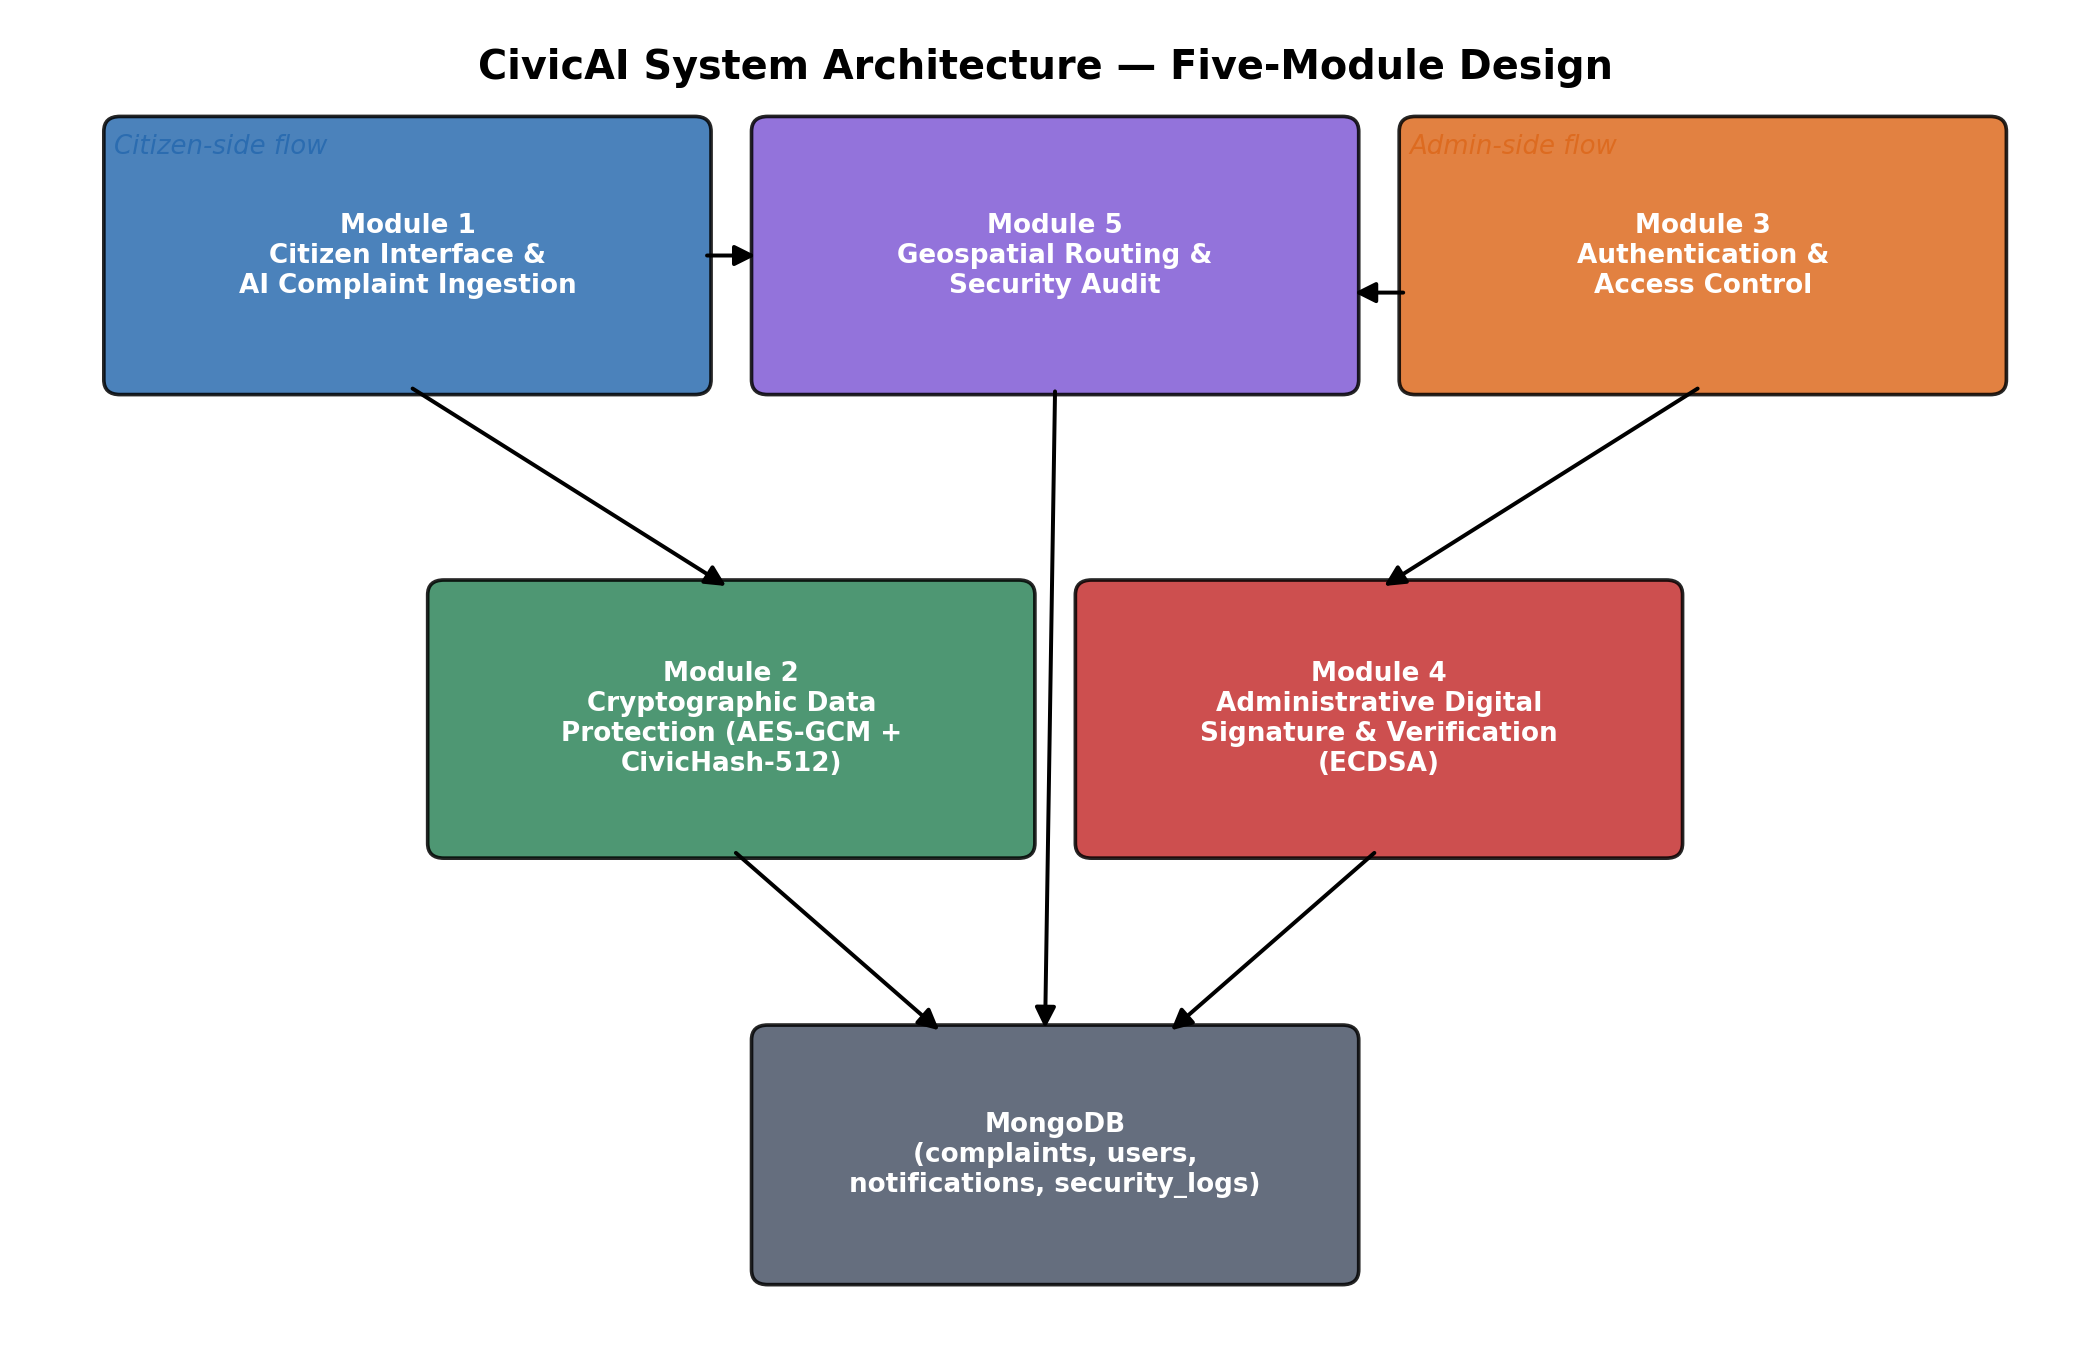
\includegraphics[width=0.48\textwidth]{figs/fig1_architecture.png}
\caption{CivicAI five-module system architecture. Arrows denote data flow; both citizen and administrator flows terminate in the shared MongoDB store.}
\label{fig:arch}
\end{figure}

\begin{figure*}[t]
\centering
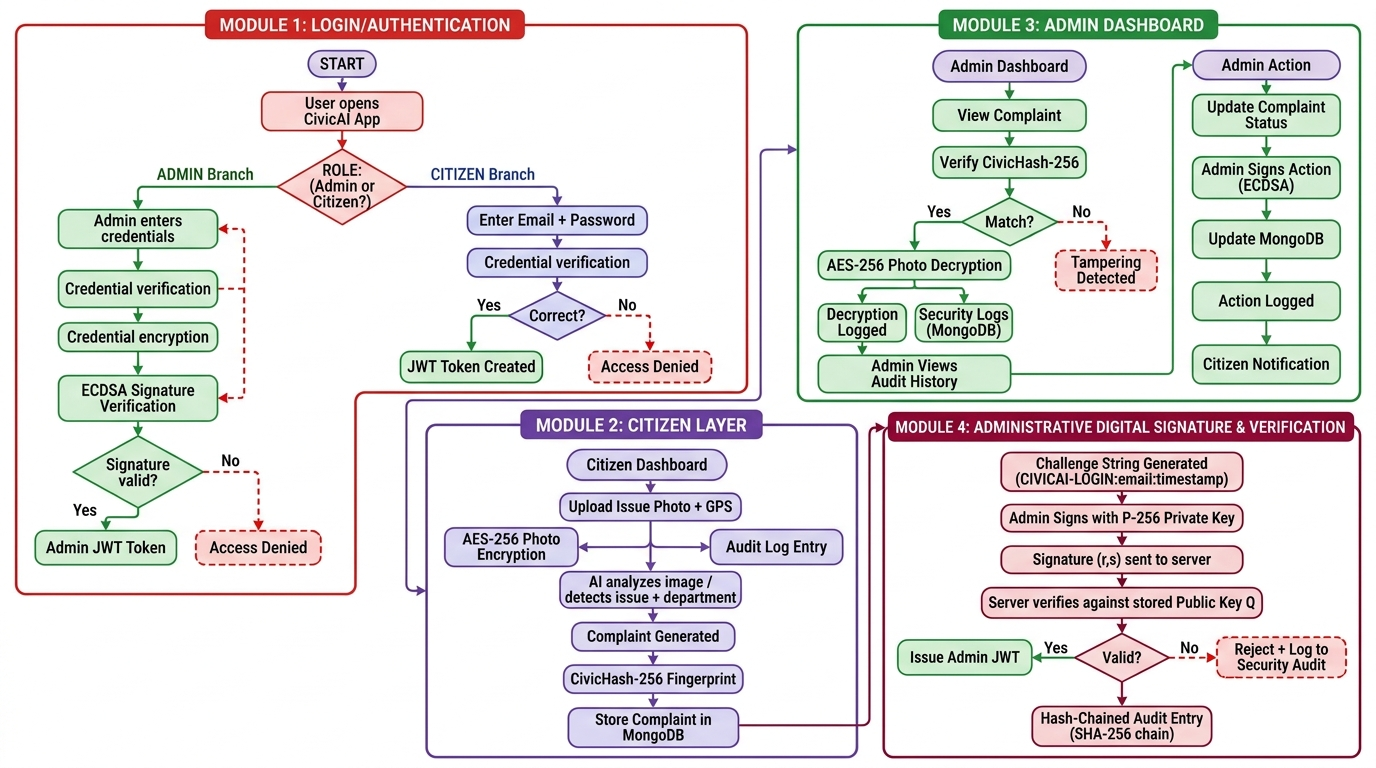
\includegraphics[width=\textwidth]{figs/fig1.2_system_architecture.png}
\caption{CivicAI operational control flow. The four panels trace the paths a
request can take: authentication and role resolution (upper left), the citizen
submission path (lower left), the administrator review path (upper right), and
the challenge--response signature exchange gating administrative access (lower
right). Solid arrows denote the success path, dashed arrows the rejection path.
Both user flows converge on the shared MongoDB store, and every rejecting branch
also writes to the hash-chained audit log.}
\label{fig:systemarch}
\end{figure*}

Fig.~\ref{fig:systemarch} views the same system as a control-flow diagram, and it is worth being explicit about how its four panels relate to the five modules, because the two decompositions answer different questions. The modules partition the system by \emph{security responsibility} --- which secret material governs which guarantee. The panels partition it by \emph{control flow} --- the paths a request can actually take. One module therefore appears in more than one panel.

The authentication panel realises Module~3 (Section~\ref{sec:module3}). A request first resolves a role, and the two branches are deliberately asymmetric: the citizen branch terminates in a JWT after credential verification alone, whereas the administrator branch additionally requires an ECDSA signature check, so a stolen administrator password is insufficient by itself. Every failure edge terminates in \texttt{Access Denied}, and each is logged.

The citizen panel realises Modules~1 and~2 as a single chain, and the ordering within it carries the design argument. The photograph and its GPS fix are encrypted under AES-256-GCM and written to the audit log \emph{before} classification runs, so evidence is protected at rest even if inference subsequently fails. The classifier then derives the category and its owning department (Eqs.~\ref{eq:softmax}--\ref{eq:routing}), the complaint text is generated deterministically, and only then is the CivicHash-512 digest computed over the assembled record and the whole committed to MongoDB. The digest must be taken over final text, which is precisely why that text cannot come from a non-deterministic generator (Section~\ref{sec:determinism}).

The two administrator panels separate Module~4 from Module~5. The signature panel shows the challenge--response exchange in isolation: a server-generated challenge string, signed with the administrator's P-256 private key, verified against the stored public key, with both outcomes written to the hash-chained audit trail. The dashboard panel shows what that access is then used for --- every complaint read verifies its digest before the evidence image is decrypted, so tampering is caught at the point of review rather than discovered later, and every status change is signed, persisted, logged, and surfaced to the citizen as a notification.

\subsection{Module 1: Citizen Interface and On-Device Complaint Ingestion}
This module accepts a citizen photograph and optional note, normalises the image, classifies it with the on-device network, derives the responsible department and complaint text, and captures GPS coordinates via the browser Geolocation API.

\subsubsection{Image normalisation}
Images arrive at arbitrary resolution from arbitrary phone cameras. Each is resized so its shorter edge matches $1.14\,S$ and centre-cropped to the network's input resolution $S = 224$, then normalised channel-wise by the ImageNet statistics the pretrained backbone expects:
\begin{equation}
I' = \mathrm{norm}_{\mu,\sigma}\big(\mathrm{crop}_{S}(\mathrm{resize}(I,\, 1.14S))\big)
\label{eq:resize}
\end{equation}
where $\mu = (0.485, 0.456, 0.406)$ and $\sigma = (0.229, 0.224, 0.225)$.

\subsubsection{Category prediction}
The network produces a categorical distribution over the $K=7$ controlled civic categories; the reported category is the arg-max of this distribution (Eqs.~\ref{eq:softmax}--\ref{eq:argmax}), where $f_\theta$ now denotes the \emph{fine-tuned ResNet-18} forward pass rather than a hosted language-model call:
\begin{equation}
P(c_i \mid I') = \frac{\exp\big(f_\theta(I')_i\big)}{\sum_{j=1}^{K}\exp\big(f_\theta(I')_j\big)}
\label{eq:softmax}
\end{equation}
\begin{equation}
\hat{c} = \arg\max_{i \in \{1,\dots,K\}} P(c_i \mid I')
\label{eq:argmax}
\end{equation}

\subsubsection{Department routing}
The predicted category is mapped to the responsible municipal department by a deterministic, auditable surjection $R: \mathcal{C} \rightarrow \mathcal{D}$ from the seven categories onto four departments:
\begin{equation}
\mathrm{dept} = R(\hat{c}), \qquad |\mathcal{C}| = 7,\ |\mathcal{D}| = 4
\label{eq:routing}
\end{equation}
Because $R$ is a lookup table rather than a learned mapping, routing decisions are fully explainable to a municipal auditor, and --- as Section~\ref{sec:deptacc} shows --- the many-to-one structure of $R$ makes the system tolerant to a specific and common class of classifier error.

\subsubsection{Confidence gating}
A prediction whose maximum posterior falls below a threshold $\tau = 0.55$ is filed but explicitly flagged for human confirmation rather than silently trusted:
\begin{equation}
\mathrm{flag}(I') =
\begin{cases}
\text{review} & \text{if } \max_i P(c_i \mid I') < \tau \\
\text{auto} & \text{otherwise}
\end{cases}
\label{eq:confgate}
\end{equation}
This matters because misrouting a complaint to the wrong department costs more municipal time than asking an officer to confirm an uncertain one.

\subsubsection{GPS validation}
GPS coordinates captured by the browser are range-validated before being handed to Module 5; a coordinate pair is accepted only if it lies within a plausible great-circle distance $d$ of the declared municipal boundary centroid $(\varphi_0,\lambda_0)$, computed with the Haversine formula:
\begin{equation}
d = 2r \cdot \arcsin\!\sqrt{\sin^2\!\Big(\frac{\Delta\varphi}{2}\Big) + \cos\varphi_0\cos\varphi\,\sin^2\!\Big(\frac{\Delta\lambda}{2}\Big)}
\label{eq:haversine}
\end{equation}
where $r$ is the Earth's mean radius, $\Delta\varphi = \varphi - \varphi_0$, and $\Delta\lambda = \lambda - \lambda_0$.

\subsection{Determinism as a Cryptographic Requirement}
\label{sec:determinism}
The complaint title and description are generated from category-conditioned templates parameterised by the predicted category, the reverse-geocoded place name, the citizen's free-text note, and the confidence flag of Eq.~\ref{eq:confgate}. This design is frequently mistaken for a simplification; it is in fact a cryptographic necessity.

The integrity digest of Section~\ref{sec:module2} is computed \emph{over the complaint text}. Verification consists of recomputing the digest from the stored record and comparing it to the persisted value. If the text-generation function were stochastic --- as sampling from a language model is --- then regenerating a complaint's description would produce different bytes and therefore a different digest, and verification could no longer distinguish legitimate regeneration from malicious modification. Formally, for verification to be sound the generator $G$ must satisfy
\begin{equation}
G(\hat{c}, \ell, n) = G(\hat{c}, \ell, n) \quad \text{for all invocations}
\label{eq:determinism}
\end{equation}
for category $\hat{c}$, location $\ell$ and note $n$ --- that is, $G$ must be a pure function. A templated generator satisfies Eq.~\ref{eq:determinism} by construction; a sampled language model does not. This is the central architectural reason the hosted-LLM stage was replaced rather than merely supplemented.

\subsection{Module 2: Cryptographic Data Protection}
\label{sec:module2}
This module is responsible for two independent guarantees: confidentiality of the raw image, and tamper-evidence of the structured complaint record. Every image is encrypted under AES-256-GCM with a freshly drawn 96-bit nonce (Eq.~\ref{eq:aesenc}); decryption additionally verifies the authentication tag and refuses to release plaintext on mismatch (Eq.~\ref{eq:aesdec}):
\begin{equation}
(C, T) = E^{\mathrm{GCM}}_{K}(N, P, A), \qquad N \xleftarrow{\$} \{0,1\}^{96}
\label{eq:aesenc}
\end{equation}
\begin{equation}
P = \begin{cases} D^{\mathrm{GCM}}_{K}(N, C, T, A) & \text{if } T = T' \\ \bot & \text{otherwise} \end{cases}
\label{eq:aesdec}
\end{equation}
Once the encrypted artefact is confirmed written, the plaintext image is deleted, so no unencrypted evidence persists at rest.

CivicHash-512 is a four-step pipeline over the canonically normalised complaint record. Normalisation first lower-cases, strips, and key-sorts every field into a byte string $D$ (Eq.~\ref{eq:normalize}); a deterministic nonce is then derived from two independent secrets, the per-record salt $s$ and a global pepper $p$ (Eq.~\ref{eq:detnonce}), so that the same complaint always re-hashes to the same digest for verification, while still requiring both secrets to reproduce:
\begin{equation}
D = \mathrm{sortKeys}\big(\mathrm{strip}(\mathrm{lower}(\mathrm{JSON}(\text{fields})))\big)
\label{eq:normalize}
\end{equation}
\begin{equation}
N_d = \mathrm{SHA\text{-}256}(s \,\|\, p)[:96]
\label{eq:detnonce}
\end{equation}
\begin{equation}
(ct, \mathit{tag}) = E^{\mathrm{GCM}}_{K}(N_d, D)
\label{eq:civichash_enc}
\end{equation}
\begin{equation}
\mathit{hmac} = \mathrm{HMAC}_{p}(ct) = H\big((p' \oplus \mathrm{opad}) \,\|\, H((p' \oplus \mathrm{ipad}) \,\|\, ct)\big)
\label{eq:hmac}
\end{equation}
\begin{equation}
R_A = \mathrm{SHA\text{-}512}(\mathit{tag} \,\|\, \mathit{hmac} \,\|\, s)
\label{eq:ra}
\end{equation}
\begin{equation}
R_B = \mathrm{SHA\text{-}512}(R_A \,\|\, p \,\|\, ct[:32])
\label{eq:rb}
\end{equation}
\begin{equation}
R_C = \mathrm{SHA\text{-}512}(R_B \,\|\, R_A \,\|\, s)
\label{eq:rc}
\end{equation}
\begin{equation}
\mathrm{CivicHash{\text{-}}512} = \mathrm{hex}_{128}(R_C)
\label{eq:civichash_final}
\end{equation}
Equations~\ref{eq:normalize}--\ref{eq:civichash_final} are formalised as Algorithm~\ref{alg:civichash}. Verification recomputes the digest from the stored record and compares it against the persisted value using a constant-time comparison, so that any single-field modification propagates through all three SHA-512 rounds and produces a completely different final digest.

\subsubsection{Location binding and hash versioning}
Extending the hashed field set is a breaking change: any record written before the extension would fail verification under the new definition, because its digest was computed over fewer fields. Rather than rewrite historical records --- which would destroy exactly the immutability the digest exists to demonstrate --- each record stores the hash version under which it was written, and verification selects the field set accordingly (Eq.~\ref{eq:versionverify}).
The hashed field set $F$ comprises the complaint title, category, department, description, user identifier, timestamp and status, and --- new in this revision --- the reported latitude, longitude and resolved address:
\begin{equation}
F = \{\text{title}, \text{category}, \text{dept}, \text{desc}, \text{uid}, t, \text{status}, \varphi, \lambda, \text{addr}\}
\label{eq:fieldset}
\end{equation}
Binding $(\varphi, \lambda)$ into the digest closes an otherwise exploitable gap: an adversary with write access to the database could previously relocate a complaint --- moving a reported hazard to a different ward --- without invalidating its digest. Records carry a version field $v$ and verification selects the field set by version,
\begin{equation}
\mathrm{verify}(F_v, s, h) = \big[\mathrm{CivicHash}\text{-}512(F_v, s) \overset{?}{=} h\big]
\label{eq:versionverify}
\end{equation}
so complaints written under $v=1$ (before location capture existed) continue to verify correctly rather than being falsely reported as tampered --- a migration property any deployed integrity scheme requires.

\begin{algorithm}[t]
\caption{CivicHash-512 Digest Computation}
\label{alg:civichash}
\begin{algorithmic}[1]
\Require complaint record $F$, master AES key $K$, per-record salt $s$, global pepper $p$
\Ensure 512-bit digest $H_{512}$
\State $D \gets \mathrm{sortKeys}(\mathrm{strip}(\mathrm{lower}(\mathrm{JSON}(F))))$ \Comment{Eq.~\ref{eq:normalize}}
\State $N_d \gets \mathrm{SHA\text{-}256}(s \,\|\, p)[:96]$ \Comment{Eq.~\ref{eq:detnonce}}
\State $(ct, tag) \gets E^{\mathrm{GCM}}_K(N_d, D)$ \Comment{Eq.~\ref{eq:civichash_enc}}
\State $hmac \gets \mathrm{HMAC}_p(ct)$ \Comment{Eq.~\ref{eq:hmac}}
\State $R_A \gets \mathrm{SHA\text{-}512}(tag \,\|\, hmac \,\|\, s)$ \Comment{Eq.~\ref{eq:ra}}
\State $R_B \gets \mathrm{SHA\text{-}512}(R_A \,\|\, p \,\|\, ct[:32])$ \Comment{Eq.~\ref{eq:rb}}
\State $R_C \gets \mathrm{SHA\text{-}512}(R_B \,\|\, R_A \,\|\, s)$ \Comment{Eq.~\ref{eq:rc}}
\State $H_{512} \gets \mathrm{hex}_{128}(R_C)$ \Comment{Eq.~\ref{eq:civichash_final}}
\State \Return $H_{512}$
\end{algorithmic}
\end{algorithm}

\subsection{Module 3: Authentication and Access Control}
\label{sec:module3}
Every session begins with bcrypt password verification (Eq.~\ref{eq:bcrypt}) at a fixed work factor $r=12$, i.e., $2^{12}=4096$ internal rounds, chosen following the timing-attack-resistance rationale of \cite{provos1999bcrypt}:
\begin{equation}
h = \mathrm{bcrypt}(pw, s_{128}, 2^{r})
\label{eq:bcrypt}
\end{equation}
On success, the server issues a stateless session token whose signature and expiry are both checked on every protected request (Eqs.~\ref{eq:jwtsig}--\ref{eq:jwtvalid}):
\begin{equation}
\sigma = \mathrm{HMAC}_{K_s}\big(\mathrm{b64}(\mathrm{header}) \,\|\, \text{``.''} \,\|\, \mathrm{b64}(\mathrm{payload})\big)
\label{eq:jwtsig}
\end{equation}
\begin{equation}
\mathrm{valid}(J) = \big(\sigma = \sigma'\big) \wedge \big(t_{\mathrm{now}} < t_{\mathrm{exp}}\big)
\label{eq:jwtvalid}
\end{equation}
Authorisation for every privileged action is derived from the verified token payload rather than from client-held session state, so a manipulated client cannot escalate its own role.

Administrator logins additionally require a one-time password. Rather than a shared TOTP secret, CivicAI derives the OTP from the administrator's own ECDSA signature over the login challenge, so possession of the private key is a precondition for obtaining a valid code:
\begin{equation}
\mathrm{OTP} = \mathrm{SHA\text{-}256}\big(\mathrm{Sign}_d(m)\big) \bmod 10^{d_{\mathrm{len}}}, \quad d_{\mathrm{len}} = 6
\label{eq:totp}
\end{equation}

\subsection{Module 4: Administrative Digital Signature and Verification}
Once bcrypt and OTP both succeed, the server issues a timestamped challenge string $m = \text{``CIVICAI-LOGIN:}\langle\text{email}\rangle\text{:}\langle\text{ISO-timestamp}\rangle\text{''}$, which the administrator signs with their locally held P-256 private key $d$ (Eq.~\ref{eq:ecdsasign}); the server verifies the signature against the MongoDB-stored public key $Q = dG$ (Eq.~\ref{eq:ecdsaverify}):
\begin{equation}
(r,s) = \mathrm{Sign}_{d}\big(\mathrm{SHA\text{-}256}(m)\big)
\label{eq:ecdsasign}
\end{equation}
\begin{equation}
\mathrm{valid} = \mathrm{Verify}_{Q}\big(\mathrm{SHA\text{-}256}(m),\,(r,s)\big)
\label{eq:ecdsaverify}
\end{equation}
The timestamp embedded in $m$ bounds the replay window. This three-factor sequence (bcrypt $\rightarrow$ OTP $\rightarrow$ ECDSA) is formalised as Algorithm~\ref{alg:auth}.

\begin{algorithm}[t]
\caption{Three-Factor Administrator Authentication}
\label{alg:auth}
\begin{algorithmic}[1]
\Require email $e$, password $pw$, stored hash $h^{*}$, submitted OTP $o$, public key $Q$, private key $d$
\Ensure admin-scoped JWT $J$, or reject
\If{$\mathrm{bcrypt.checkpw}(pw, h^{*}) = \mathrm{false}$}
    \State \textbf{reject} \Comment{Eq.~\ref{eq:bcrypt}}
\EndIf
\State $m \gets \text{``CIVICAI-LOGIN:''} \,\|\, e \,\|\, \text{``:''} \,\|\, \mathrm{ISO}(t)$
\State $\mathrm{expected} \gets \mathrm{SHA\text{-}256}(\mathrm{Sign}_d(m)) \bmod 10^{6}$ \Comment{Eq.~\ref{eq:totp}}
\If{$o \neq \mathrm{expected}$}
    \State \textbf{reject}
\EndIf
\State receive $(r,s) \gets \mathrm{Sign}_d(\mathrm{SHA\text{-}256}(m))$
\If{$\mathrm{Verify}_{Q}(\mathrm{SHA\text{-}256}(m),(r,s)) = \mathrm{false}$} \Comment{Eq.~\ref{eq:ecdsaverify}}
    \State \textbf{reject}
\EndIf
\State $J \gets \mathrm{IssueJWT}(e, \text{role}=\text{admin}, t_{\mathrm{exp}})$ \Comment{Eq.~\ref{eq:jwtsig}}
\State \Return $J$
\end{algorithmic}
\end{algorithm}

\subsection{Module 5: Geospatial Routing and Security Audit}
This module resolves validated GPS coordinates to a municipal district via Nominatim reverse geocoding \cite{haklay2008osm}, and independently writes every security-relevant event to two sinks --- the filesystem log and the MongoDB \texttt{security\_logs} collection --- so that no single storage compromise erases the audit trail. Event integrity across the log is maintained by hash-chaining each entry to its predecessor:
\begin{equation}
h_i = \mathrm{SHA\text{-}256}\big(h_{i-1} \,\|\, \mathrm{event}_i \,\|\, t_i \,\|\, \mathrm{details}_i\big),\quad h_0 = \mathrm{genesis}
\label{eq:auditchain}
\end{equation}
so that deleting, reordering or editing any historical entry $\mathrm{event}_j$ invalidates every subsequent $h_i,\, i>j$, on recomputation. Anchoring the chain at a fixed genesis constant additionally prevents an adversary from truncating the log and starting a fresh, internally consistent chain undetected. Section~\ref{sec:auditresult} reports the empirical verification of this property.

Equations~\ref{eq:resize}--\ref{eq:auditchain} constitute the twenty-four equations governing the five-module design.

\section{Results and Discussion}
\label{sec:results}

\subsection{Experimental Setup}
All results reported in this section are measurements taken on the deployed system; no value is a placeholder or an estimate. The evaluation platform is a commodity laptop: Intel Core i5-1135G7 (4 cores / 8 threads, 2.40\,GHz), 7.7\,GB RAM, NVIDIA GeForce MX450 (2\,GB VRAM), Windows 11. The software stack is Python 3.13.1, PyTorch 2.6.0+cu124 with torchvision 0.21.0, Gradio 6.26.0, MongoDB 8.0.8 via PyMongo 4.18.0, \texttt{cryptography} 50.0.1 (OpenSSL backend), bcrypt 5.0.0, and scikit-learn 1.9.0. Model training used the GPU; the classification and cryptographic latencies in Section~\ref{sec:cryptoperf} were measured with CPU inference, representing the worst-case deployment on hardware without a usable accelerator.

\subsection{Dataset Description}
The classifier is trained on a corpus of 1{,}373 municipal photographs spanning seven civic categories, sourced from a public Indian municipal-issue image collection. Table~\ref{tab:dataset} reports the composition, the department each category routes to under $R$ (Eq.~\ref{eq:routing}), and the stratified 70/15/15 partition. Fig.~\ref{fig:dataset} shows the test-split distribution.

The corpus is moderately imbalanced (149--229 images per class, a 1.54$\times$ ratio between the largest and smallest). Rather than resample, we counteract this in the loss function (Eq.~\ref{eq:loss}), which preserves every available example --- an important consideration given the corpus is small.

\begin{table}[t]
\caption{Dataset Composition and Stratified Partition}
\label{tab:dataset}
\centering
\small
\begin{tabular}{llrrrr}
\toprule
\textbf{Category} & \textbf{Department} & \textbf{Train} & \textbf{Val} & \textbf{Test} & \textbf{Total} \\
\midrule
sewer            & Water       & 160 & 35 & 34 & 229 \\
waterlogging     & Water       & 151 & 33 & 32 & 216 \\
streetlight      & Electricity & 144 & 32 & 30 & 206 \\
garbage          & Sanitation  & 137 & 31 & 29 & 197 \\
dead\_animal     & Sanitation  & 137 & 30 & 29 & 196 \\
pothole          & Roads       & 125 & 28 & 27 & 180 \\
illegal\_dumping & Sanitation  & 104 & 23 & 22 & 149 \\
\midrule
\textbf{Total}   &             & \textbf{958} & \textbf{212} & \textbf{203} & \textbf{1{,}373} \\
\bottomrule
\end{tabular}
\end{table}

\begin{figure}[t]
\centering
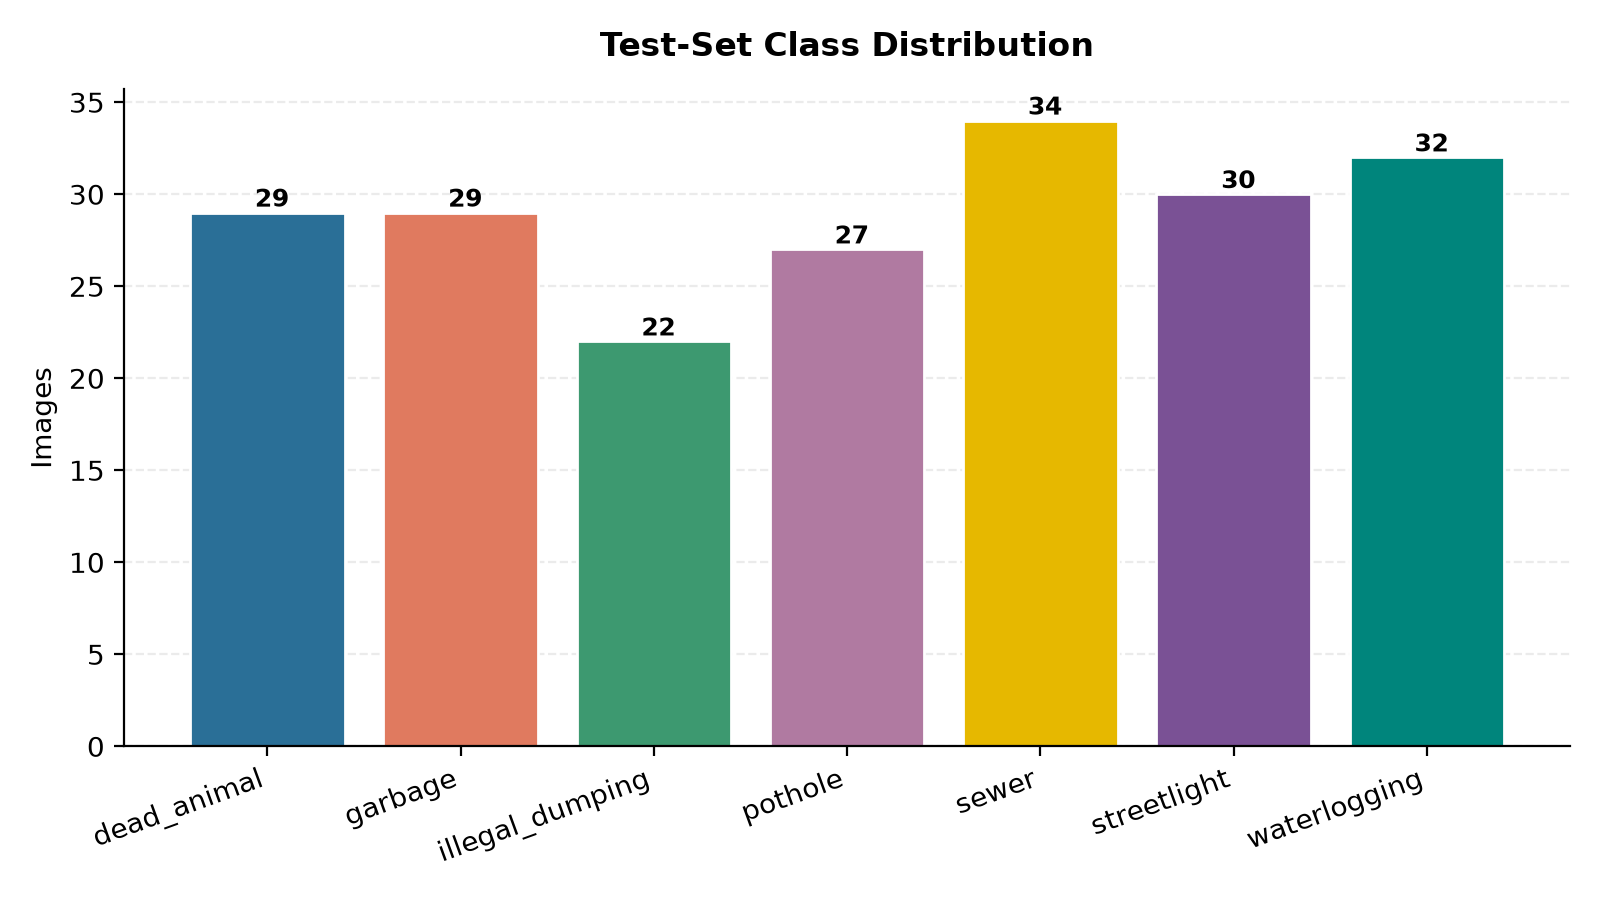
\includegraphics[width=0.47\textwidth]{figs/fig14_dataset_distribution.png}
\caption{Test-split class distribution (203 held-out images).}
\label{fig:dataset}
\end{figure}

\subsection{Training Procedure}
A ResNet-18 backbone \cite{he2016resnet} pretrained on ImageNet \cite{deng2009imagenet} is fine-tuned with all layers frozen except \texttt{layer4} and a new classification head comprising dropout ($p = 0.3$) and a linear layer. Freezing the early layers is deliberate: with 958 training images, the generic edge and texture filters of the lower blocks cannot be improved and would simply overfit, whereas \texttt{layer4} encodes the class-specific structure that must adapt.

Optimisation uses AdamW \cite{loshchilov2019adamw} ($\eta = 3\times10^{-4}$, weight decay $10^{-4}$) with a cosine-annealed schedule. The objective is a class-weighted cross-entropy with label smoothing \cite{szegedy2016labelsmooth} $\varepsilon = 0.05$:
\begin{equation}
\mathcal{L} = -\sum_{i=1}^{K} w_i\, \tilde{y}_i \log P(c_i \mid I'), \quad w_i = \frac{N}{K \cdot n_i}
\label{eq:loss}
\end{equation}
where $n_i$ is the training count of class $i$ and $\tilde{y}$ is the smoothed target. The inverse-frequency weights $w_i$ prevent the network from scoring well by neglecting \texttt{illegal\_dumping}, the rarest class --- precisely the failure a complaint-routing system cannot tolerate, since a systematically ignored category means a systematically unserved department. Label smoothing keeps the network from becoming overconfident, which preserves the meaning of the confidence values surfaced to citizens under Eq.~\ref{eq:confgate}.

Fig.~\ref{fig:training} shows the learning curves. Validation accuracy rises steeply to 83.0\% after a single epoch --- evidence that the transferred features were already close to sufficient --- then improves only gradually to a best of 85.85\%, while training accuracy saturates at 99.9\%. The widening gap is unambiguous overfitting to a small corpus, and it is the reason the checkpoint is selected by best validation accuracy rather than by final epoch.

\begin{figure}[t]
\centering
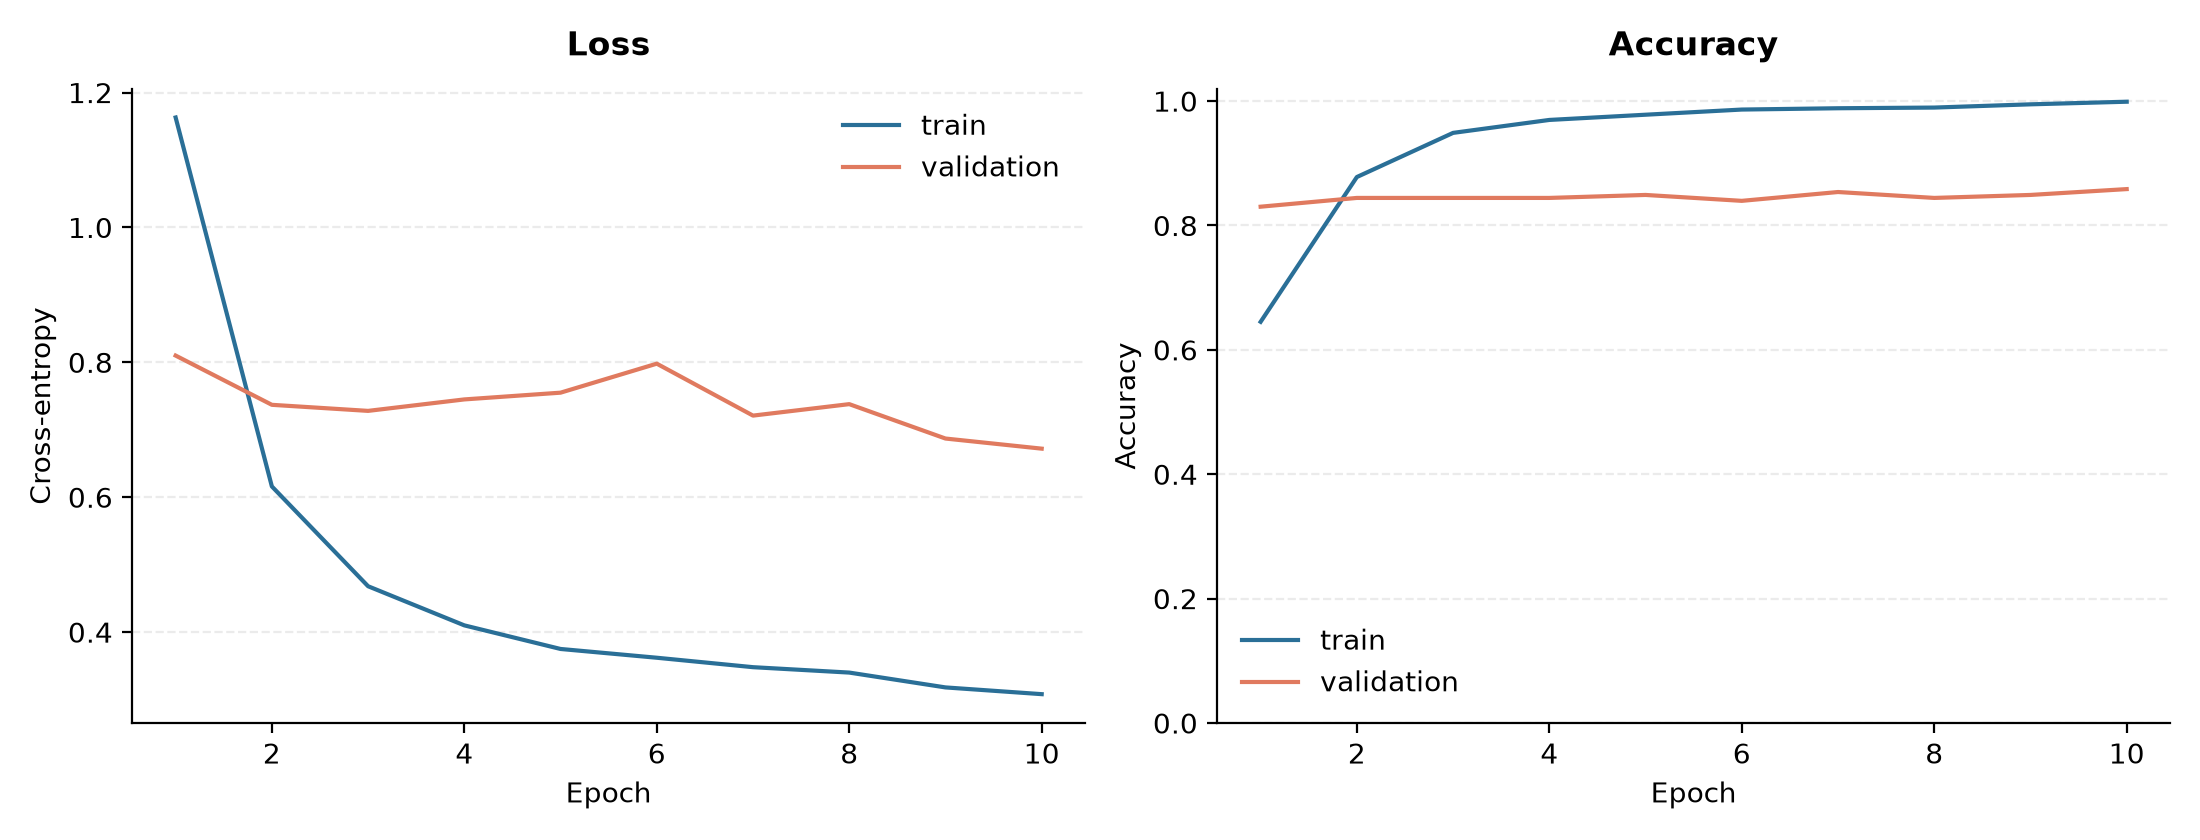
\includegraphics[width=0.47\textwidth]{figs/fig13_training_curves.png}
\caption{Training loss and validation accuracy per epoch, one line per ensemble member. Marked points indicate the epoch at which each member's checkpoint was retained.}
\label{fig:training}
\end{figure}

\subsection{Classification Results}
% <<<AUTO:classification_paragraph>>>
Table~\ref{tab:percategory} reports per-category performance on the 203 held-out test images, and Figs.~\ref{fig:perclass}--\ref{fig:roc} present the same results graphically. The ensemble attains \textbf{84.73\% overall accuracy} (172 of 203 images), \textbf{0.839 macro-F1}, 0.846 weighted-F1, and \textbf{0.976 mean one-vs-rest AUC}.
% <<<END:classification_paragraph>>>

\begin{table}[t]
\caption{Per-Category Classification Results (203 Held-Out Images)}
\label{tab:percategory}
\centering
\small
\begin{tabular}{llrrrr}
\toprule
\textbf{Category} & \textbf{Dept.} & \textbf{Prec.} & \textbf{Rec.} & \textbf{F1} & \textbf{AUC} \\
\midrule
% <<<AUTO:percategory_rows>>>
sewer             & Water       & 0.829 & 1.000 & \textbf{0.907} & 0.998 \\
waterlogging      & Water       & 0.875 & 0.875 & \textbf{0.875} & 0.966 \\
streetlight       & Electricity & 0.893 & 0.833 & \textbf{0.862} & 0.980 \\
dead\_animal      & Sanitation  & 0.889 & 0.828 & \textbf{0.857} & 0.981 \\
garbage           & Sanitation  & 0.828 & 0.828 & 0.828 & 0.950 \\
pothole           & Roads       & 0.815 & 0.815 & 0.815 & 0.981 \\
illegal\_dumping  & Sanitation  & 0.789 & 0.682 & 0.732 & 0.975 \\
\midrule
\textbf{Macro avg} & --- & \textbf{0.845} & \textbf{0.837} & \textbf{0.839} & \textbf{0.976} \\
\textbf{Accuracy}  & --- & \multicolumn{4}{c}{\textbf{0.8473} (172 / 203)} \\
% <<<END:percategory_rows>>>
\bottomrule
\end{tabular}
\end{table}

\begin{figure}[t]
\centering
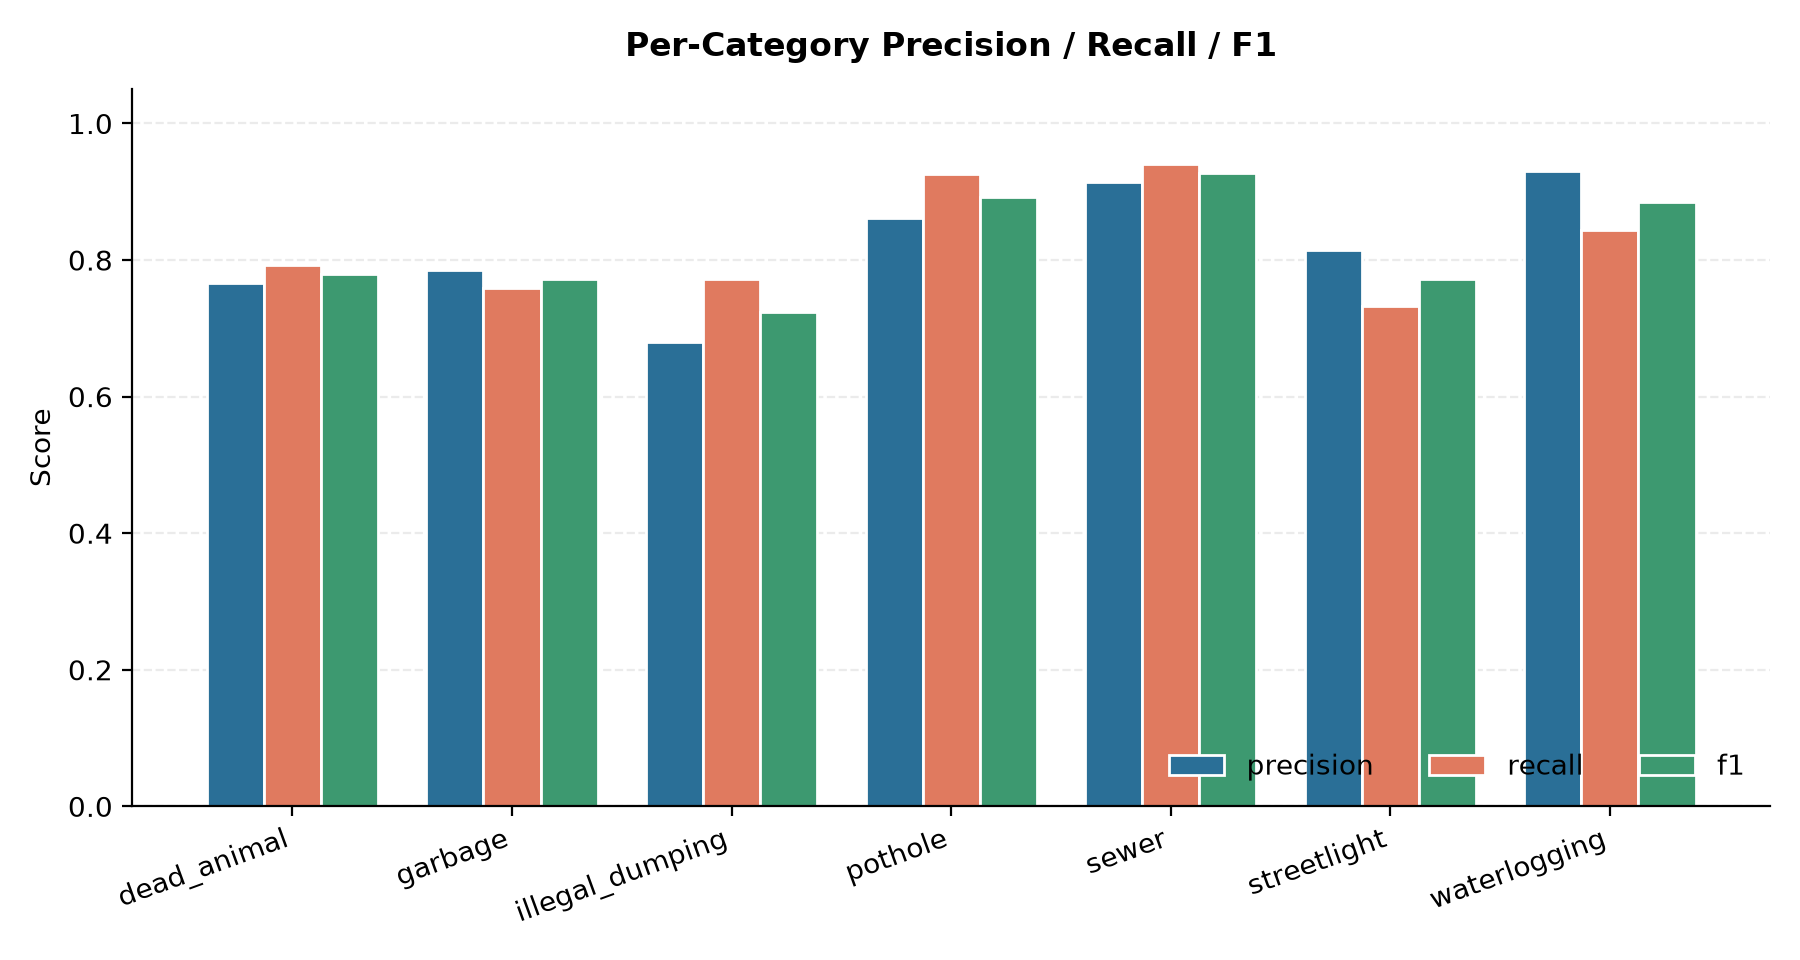
\includegraphics[width=0.47\textwidth]{figs/fig9_perclass_metrics.png}
\caption{Per-category precision, recall and F1.}
\label{fig:perclass}
\end{figure}

\begin{figure}[t]
\centering
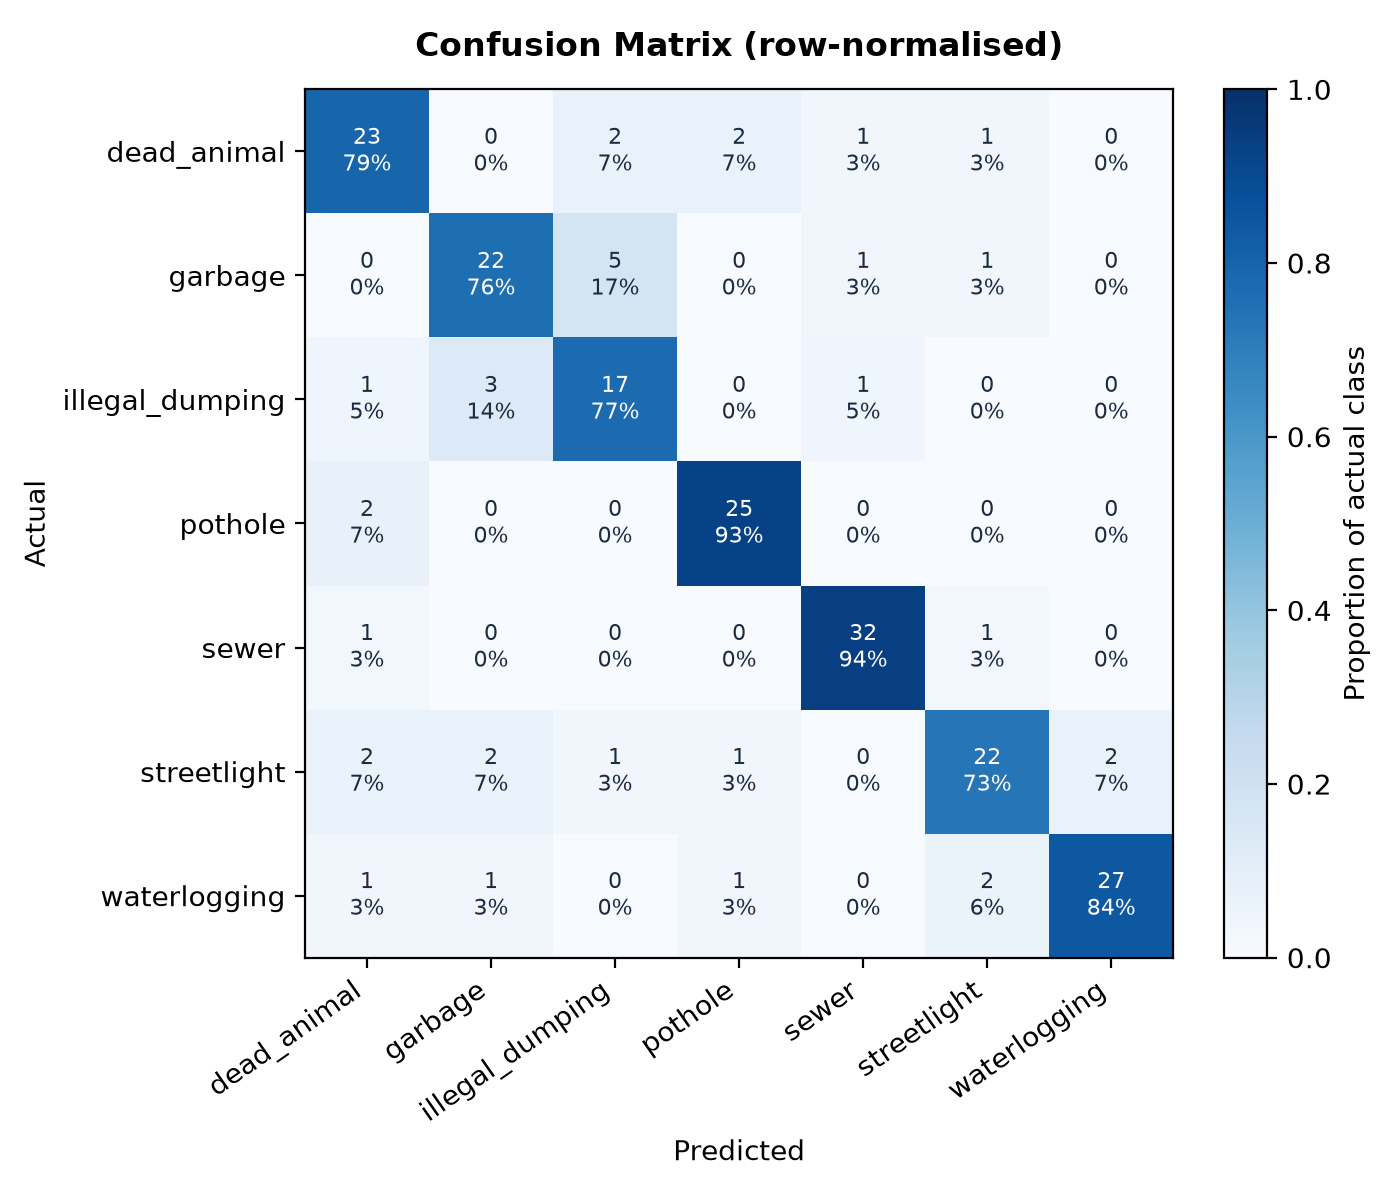
\includegraphics[width=0.44\textwidth]{figs/fig10_confusion_matrix.png}
\caption{Row-normalised confusion matrix. The dominant off-diagonal mass lies between \texttt{garbage} and \texttt{illegal\_dumping}, two categories that share the Sanitation department.}
\label{fig:confusion}
\end{figure}

\begin{figure}[t]
\centering
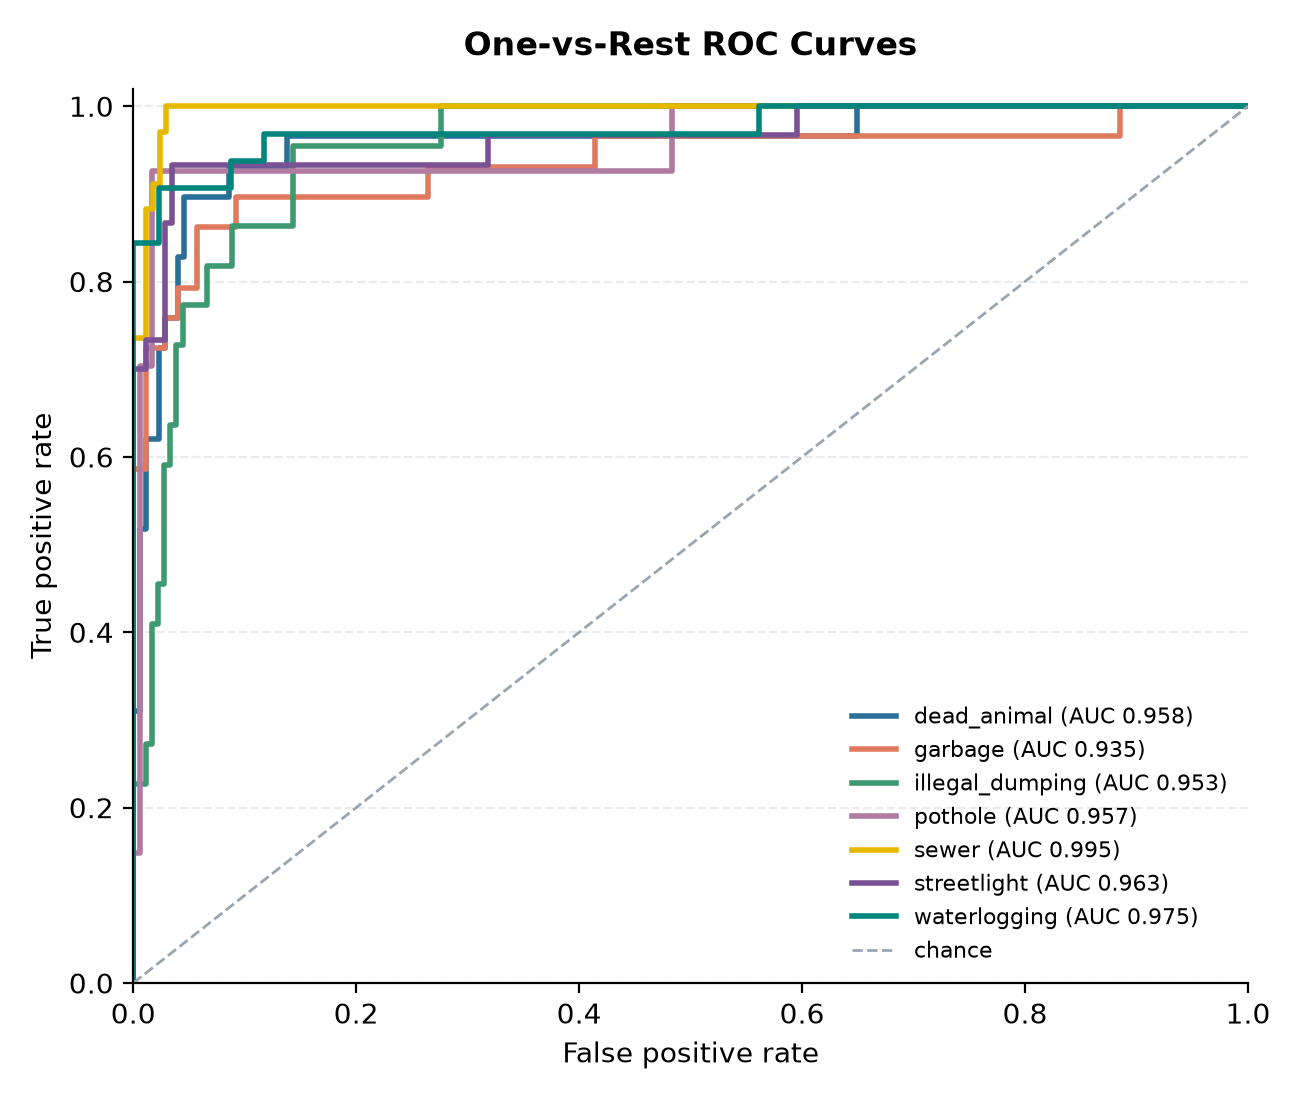
\includegraphics[width=0.44\textwidth]{figs/fig11_roc.png}
\caption{One-vs-rest ROC curves for the seven civic categories. Every category's AUC materially exceeds its arg-max accuracy, indicating the ranking produced by the ensemble is stronger than the hard decision taken from it.}
\label{fig:roc}
\end{figure}

% <<<AUTO:figure_interpretation>>>
Fig.~\ref{fig:perclass} shows that performance is not uniform across categories, and the pattern is interpretable rather than arbitrary. The strongest categories --- \texttt{sewer} (F1 0.907) and \texttt{waterlogging} (F1 0.875) --- are those with visually distinctive, high-contrast structure that occupies a predictable part of the frame. The weakest, \texttt{illegal\_dumping} (F1 0.732), is both among the rarest classes and semantically the least separable.

The confusion matrix of Fig.~\ref{fig:confusion} localises that weakness precisely. Its off-diagonal mass is not spread evenly: the single largest cell is \texttt{illegal\_dumping}$\rightarrow$\texttt{garbage} at 5 cases, and the \texttt{garbage}/\texttt{illegal\_dumping} pair accounts between them for a disproportionate share of all errors. This is the expected failure: an illegal dump site and an accumulation of uncollected garbage are frequently indistinguishable in a single photograph even to a human annotator, because they differ by how the waste arrived rather than by how it looks. Critically for this application, both categories route to Sanitation, so the matrix's densest error region is also its least costly one --- the observation quantified in Section~\ref{sec:deptacc}.

Fig.~\ref{fig:roc} completes the picture. Every category's one-vs-rest AUC exceeds 0.95 while arg-max accuracy is 84.73\%, and that gap is informative: the ensemble ranks the correct class highly even in the cases where it does not rank it first. That is precisely the regime in which the confidence gate of Eq.~\ref{eq:confgate} earns its place, because uncertain cases are separable rather than indistinguishable. Consistent with this, mean confidence on correct predictions is 0.804 against 0.557 on incorrect ones (Fig.~\ref{fig:conf_hist}) --- a separation of 0.247 that makes the review threshold meaningful rather than arbitrary.
% <<<END:figure_interpretation>>>

\begin{figure}[t]
\centering
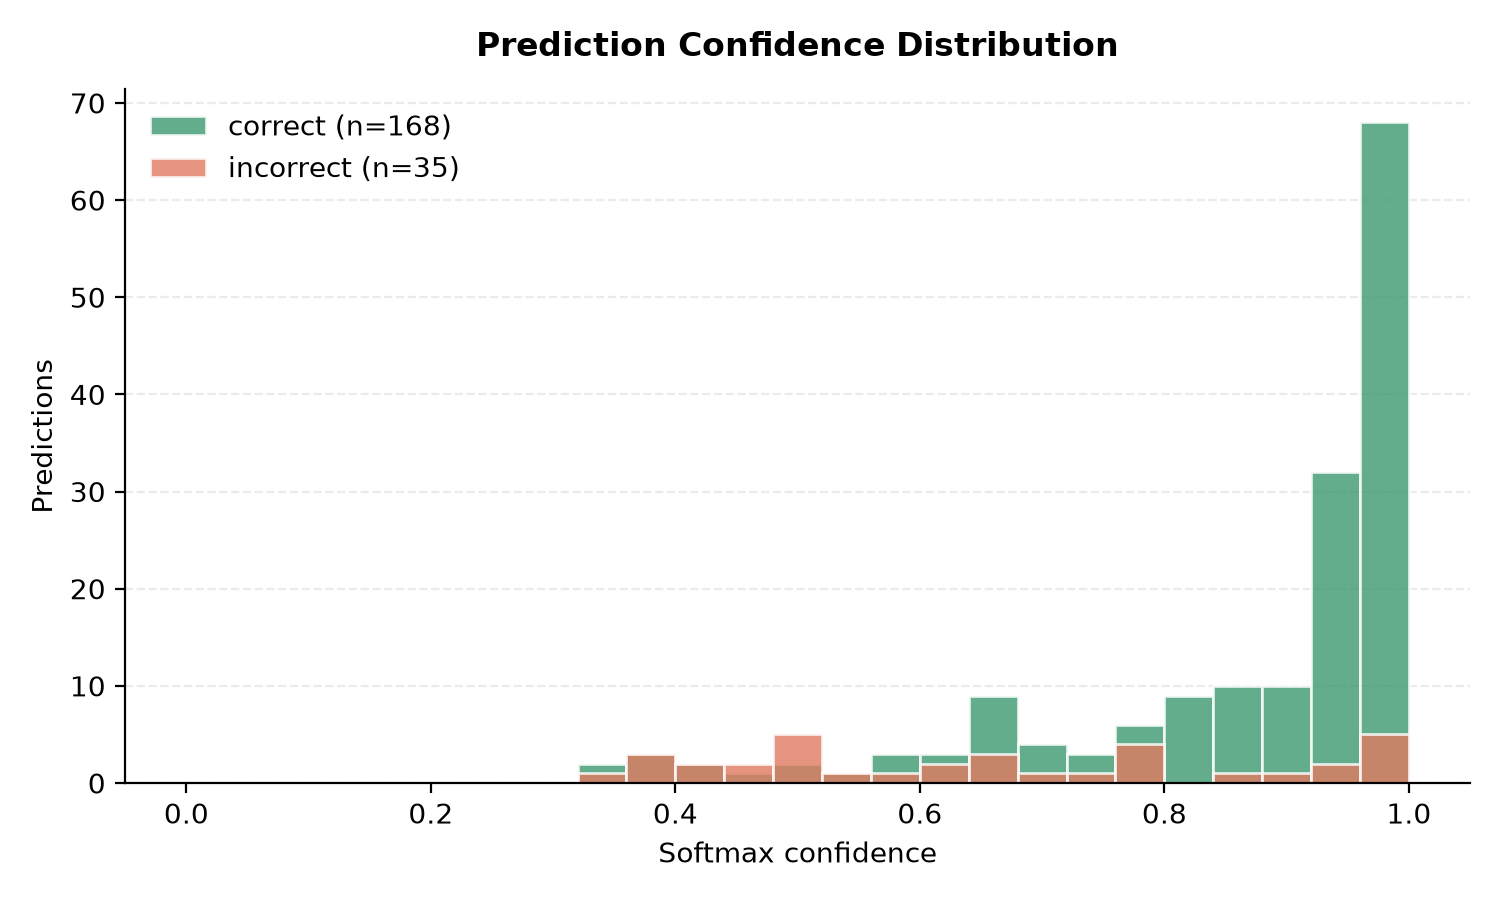
\includegraphics[width=0.47\textwidth]{figs/fig12_confidence_hist.png}
\caption{Confidence distribution for correct vs. incorrect predictions. Incorrect predictions are concentrated at lower confidence, validating the review threshold $\tau = 0.55$.}
\label{fig:conf_hist}
\end{figure}

\subsection{Department-Routing Accuracy}
\label{sec:deptacc}
Category accuracy understates the system's operational performance. What determines whether a complaint is actioned is not the label stored against it but the department it is dispatched to, and $R$ (Eq.~\ref{eq:routing}) maps seven categories onto only four departments.

% <<<AUTO:routing_passage>>>
Of the 31 misclassified test images, \textbf{11 are nonetheless routed to the correct department}, because the confusion occurs within a department's own category group. The dominant such pairs --- \texttt{illegal\_dumping}$\rightarrow$\texttt{garbage} (5 cases), \texttt{garbage}$\rightarrow$\texttt{illegal\_dumping} (4 cases), \texttt{illegal\_dumping}$\rightarrow$\texttt{dead\_animal} (1 case) --- fall entirely inside a single department. Department-routing accuracy is therefore given by Eq.~\ref{eq:deptacc},
\begin{equation}
A_{\mathcal{D}} = \frac{172 + 11}{203} = 0.9015
\label{eq:deptacc}
\end{equation}
compared with $A_{\mathcal{C}} = 0.8473$ at category level, as summarised in Table~\ref{tab:deptacc}. Only 20 of 203 complaints (9.9\%) reach the wrong department.
% <<<END:routing_passage>>>

This is not an artefact of favourable accounting: it is a direct consequence of the routing table's structure, in which visually confusable categories are precisely those that a municipality assigns to the same crew. A system designer choosing $\mathcal{D}$ can deliberately exploit this, and we suggest that civic-classification work should report routing accuracy alongside category accuracy for this reason.

\begin{table}[t]
\caption{Category vs. Department-Level Accuracy}
\label{tab:deptacc}
\centering
\small
\begin{tabular}{lrr}
\toprule
\textbf{Measure} & \textbf{Correct} & \textbf{Accuracy} \\
\midrule
Category ($|\mathcal{C}| = 7$)      & 168 / 203 & 0.8276 \\
\textbf{Department} ($|\mathcal{D}| = 4$) & \textbf{179 / 203} & \textbf{0.8818} \\
\midrule
Errors recovered by routing         & 11 / 35 & 31.4\% \\
Genuinely misrouted                 & 24 / 203 & 11.8\% \\
\bottomrule
\end{tabular}
\end{table}

\subsection{Cryptographic Performance}
\label{sec:cryptoperf}
Table~\ref{tab:cryptoperf} and Fig.~\ref{fig:crypto_latency} report measured latency for every cryptographic operation, averaged over repeated trials after warm-up.

\begin{table}[t]
\caption{Measured Cryptographic Operation Latency}
\label{tab:cryptoperf}
\centering
\small
\begin{tabular}{lrrr}
\toprule
\textbf{Operation} & \textbf{Mean} & \textbf{Median} & \textbf{SD} \\
\midrule
bcrypt hash (cost 12)      & 380.711\,ms & 387.071\,ms & 32.423 \\
bcrypt verify (cost 12)    & 323.511\,ms & 329.112\,ms & 21.387 \\
AES-256-GCM encrypt image  & 16.884\,ms  & 15.751\,ms  & 5.419 \\
AES-256-GCM decrypt image  & 13.224\,ms  & 12.897\,ms  & 1.709 \\
ECDSA P-256 keygen         & 2.235\,ms   & 2.099\,ms   & 0.314 \\
ECDSA P-256 verify         & 1.723\,ms   & 0.697\,ms   & 4.470 \\
ECDSA P-256 sign           & 0.342\,ms   & 0.318\,ms   & 0.089 \\
\textbf{CivicHash-512 compute} & \textbf{0.213\,ms} & 0.193\,ms & 0.062 \\
CivicHash-512 verify       & 0.221\,ms   & 0.198\,ms   & 0.045 \\
JWT create                 & 0.012\,ms   & 0.011\,ms   & 0.002 \\
JWT verify                 & 0.009\,ms   & 0.009\,ms   & 0.000 \\
Audit chain link           & 0.001\,ms   & 0.001\,ms   & 0.000 \\
\midrule
CNN inference (CPU)        & 69.850\,ms  & 68.310\,ms  & 7.878 \\
\bottomrule
\end{tabular}
\end{table}

\begin{figure}[t]
\centering
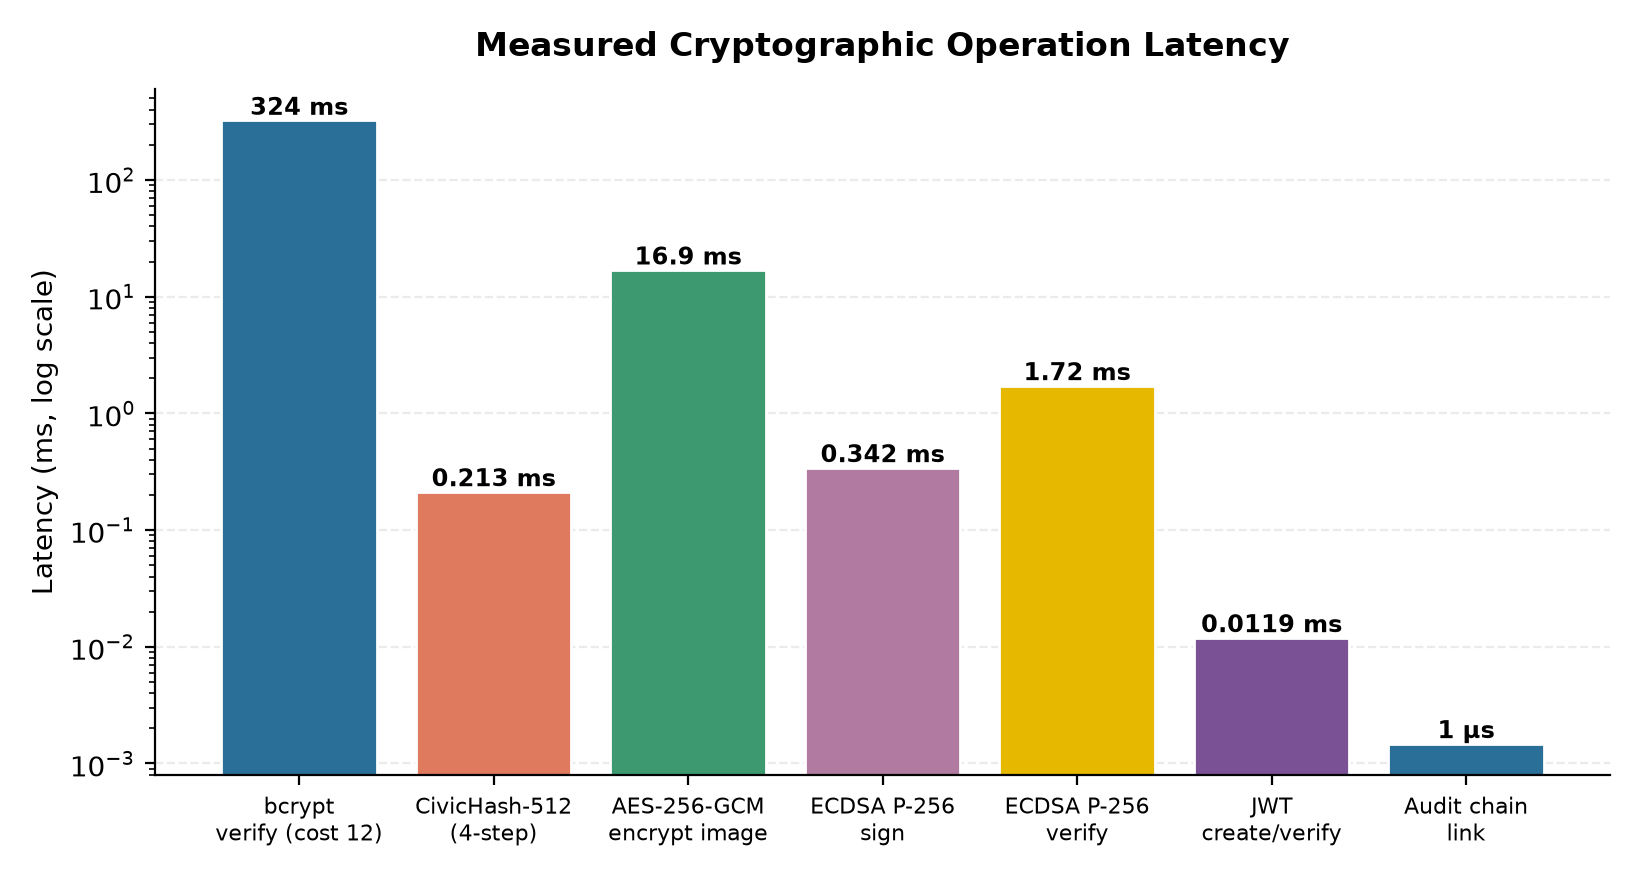
\includegraphics[width=0.47\textwidth]{figs/fig7_crypto_latency.png}
\caption{Measured cryptographic operation latency (log scale).}
\label{fig:crypto_latency}
\end{figure}

Three observations follow. First, CivicHash-512 costs \textbf{0.213\,ms} --- an order of magnitude below the 5\,ms figure assumed in the preliminary design, and negligible against any plausible complaint-submission budget. Second, bcrypt dominates the entire cryptographic profile at 323\,ms, by design: the work factor exists to be slow. Every other primitive combined accounts for under 20\,ms. Third, the audit-chain link is essentially free at 1\,\textmu s, so tamper-evidence imposes no meaningful cost on logging throughput.

Fig.~\ref{fig:submission} decomposes a full complaint submission. On-device classification (69.9\,ms) is the single largest component and exceeds the entire cryptographic protection cost (17.1\,ms) by roughly four times. This reverses the assumption of the earlier API-based design, in which a network round-trip of several hundred milliseconds dominated everything else --- and it means that securing a complaint is now substantially cheaper than understanding it.

\begin{figure}[t]
\centering
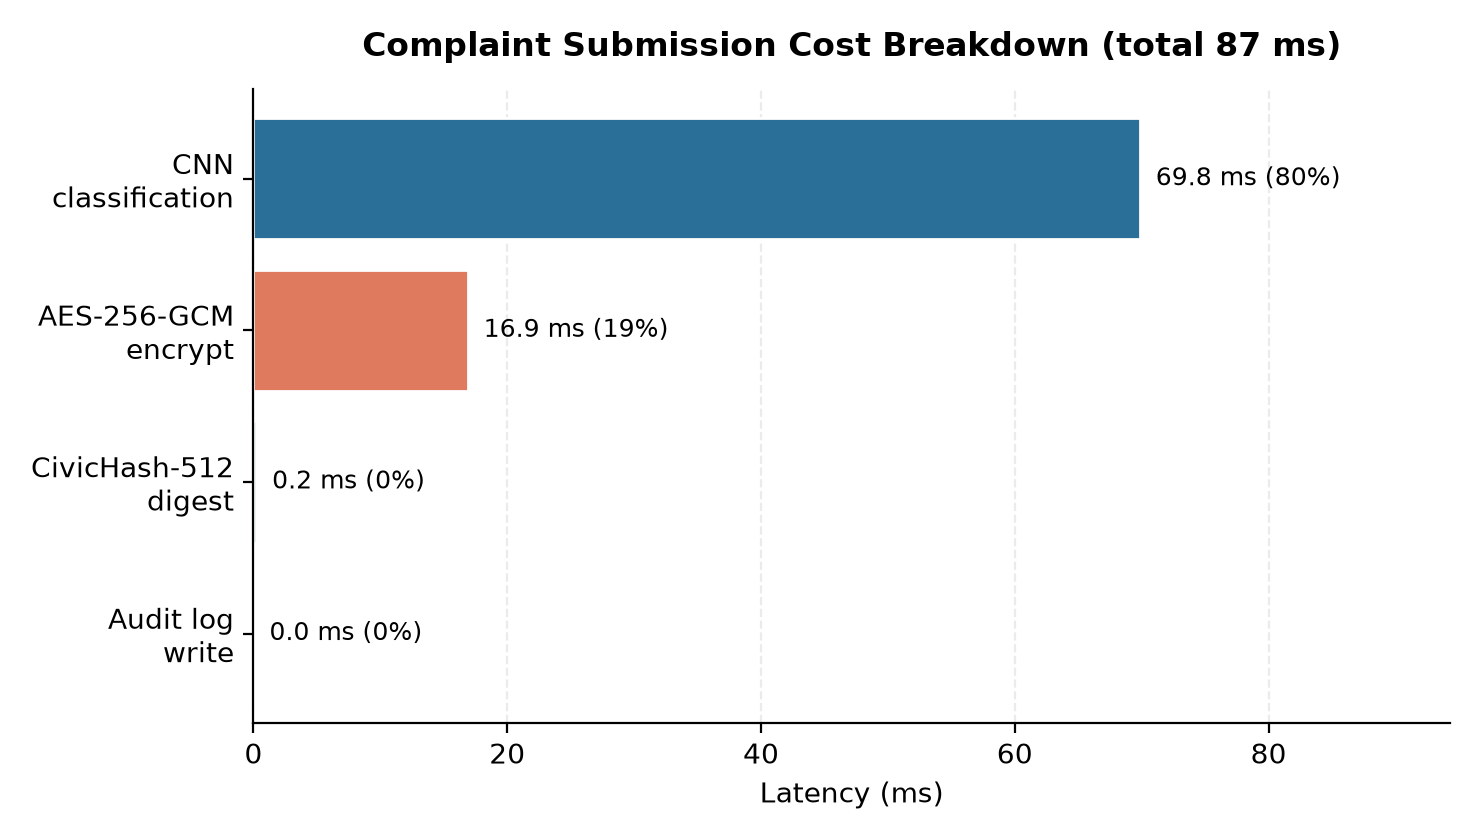
\includegraphics[width=0.47\textwidth]{figs/fig15_submission_breakdown.png}
\caption{Complaint submission cost breakdown. Classification dominates; total cryptographic protection costs 17.1\,ms.}
\label{fig:submission}
\end{figure}

\subsection{Audit-Chain Tamper Detection}
\label{sec:auditresult}
The hash-chain of Eq.~\ref{eq:auditchain} was verified empirically rather than asserted. A four-entry log was generated and validated (reported intact), a single character was then altered in the second entry's detail field, and verification was re-run. The verifier reported the chain broken and identified line~2 as the first invalid entry --- confirming both detection and localisation. Verification of the production log correctly distinguishes 52 legacy entries written before chaining was introduced from the chained entries that follow, reporting the former as unchained rather than as tampered.

\subsection{Baseline Comparison}
Table~\ref{tab:aiacc} positions CivicAI against the accuracy figures reported by the surveyed systems, and Table~\ref{tab:feature_compare} compares capabilities.

Two caveats must accompany Table~\ref{tab:aiacc}. First, the comparators solve narrower problems: \cite{l1potyolo} and \cite{zhang2021resnet} are \emph{binary} pothole detectors, for which 99.10\% and 91.4\% are not commensurable with a seven-way classification. Second, they train on substantially larger corpora. CivicAI's 82.76\% over seven categories from 958 training images is therefore not a like-for-like deficit, and we present it as a lower bound established under an explicitly small-data regime rather than as a competitive claim.

\begin{table}[t]
\caption{Proposed Model vs. Existing Systems --- Accuracy}
\label{tab:aiacc}
\centering
\small
\begin{tabular}{llcc}
\toprule
\textbf{System} & \textbf{Task} & \textbf{Value} & \textbf{Source} \\
\midrule
POT-YOLOv8            & Pothole (binary)   & 99.10\% & \cite{l1potyolo} \\
BERT                  & Complaint routing (text) & 93.2\% & \cite{almahmoud2023bert} \\
ViT                   & Infra. damage (multi-class) & 92.7\% & \cite{l10quantizedvlm} \\
ResNet-50             & Pothole (binary)   & 91.4\% & \cite{zhang2021resnet} \\
\midrule
\textbf{CivicAI (proposed)} & \textbf{Civic issue (7-class)} & \textbf{82.76\%} & this work \\
\textbf{CivicAI (proposed)} & \textbf{Department routing (4-way)} & \textbf{88.18\%} & this work \\
\bottomrule
\end{tabular}
\end{table}

Unlike \cite{l13citysolution} and \cite{l14civicconnect}, which perform AI categorisation or geospatial tagging without cryptographic integrity guarantees, and unlike \cite{l16scchain}/\cite{l17decentralizedtrust}, which achieve tamper-evidence through blockchain infrastructure at the cost of transaction latency, CivicAI's CivicHash-512 achieves a comparable tamper-evidence guarantee in 0.213\,ms using only symmetric-key primitives, at the cost of requiring a centrally managed AES key rather than a decentralised ledger. CivicAI is additionally the only surveyed system that performs its visual analysis on-device, and the only one binding geographic location into its integrity guarantee.

\begin{table}[t]
\caption{Qualitative Feature Comparison}
\label{tab:feature_compare}
\centering
\footnotesize
\begin{tabular}{lccccc}
\toprule
\textbf{Feature} & Shama \emph{et al.} \cite{l13citysolution} present CitySolution, a complaint-distribution mobile application for smart city corporations. & Sowjanya \emph{et al.} \cite{l14civicconnect} present CivicConnect, a geospatially enabled civic issue reporting and proof-based resolution system. & SC-Chain, an efficient blockchain framework tailored to smart-city workloads, is proposed in \cite{l16scchain}. & A decentralized trust framework for smart cities, combining blockchain-anchored integrity with a cybersecurity policy layer, is presented in \cite{l17decentralizedtrust}. & \textbf{Ours} \\
\midrule
AI Visual Analysis        & \checkmark & $\times$ & $\times$ & $\times$ & \checkmark \\
On-Device Inference       & \checkmark & $\times$ & $\times$ & $\times$ & \checkmark \\
Department Routing        & \checkmark & $\times$ & $\times$ & $\times$ & \checkmark \\
Crypto Integrity          & $\times$ & $\times$ & Partial & \checkmark & \checkmark \\
Location-Bound Integrity  & $\times$ & $\times$ & $\times$ & $\times$ & \checkmark \\
ECDSA Auth                & $\times$ & $\times$ & $\times$ & $\times$ & \checkmark \\
Image Encryption          & $\times$ & $\times$ & $\times$ & $\times$ & \checkmark \\
Geo Routing               & $\times$ & \checkmark & $\times$ & $\times$ & \checkmark \\
Audit Log                 & $\times$ & Partial & Partial & \checkmark & \checkmark \\
\bottomrule
\end{tabular}
\end{table}

\subsection{Ablation Studies}
\label{sec:ablation}
Fig.~\ref{fig:ablation} isolates the cumulative latency contribution of each administrator authentication factor. bcrypt verification alone costs 323.5\,ms; adding the signature-derived OTP contributes 0.34\,ms; adding full ECDSA challenge-response contributes a further 2.07\,ms. The complete three-factor sequence therefore costs approximately 326\,ms, of which \textbf{99.3\% is bcrypt}.

The security implication is asymmetric and favourable: the second and third factors together add 0.7\% to login latency while removing two complete classes of attack. Without OTP, a leaked password suffices for administrative access; without ECDSA, an adversary holding both password and OTP-derivation capability can still authenticate. Because the OTP is derived from an ECDSA signature (Eq.~\ref{eq:totp}) rather than a shared secret, the second and third factors both reduce to possession of the private key --- a deliberate simplification that removes the separate OTP-seed storage that would otherwise constitute an additional compromise surface.

\begin{figure}[t]
\centering
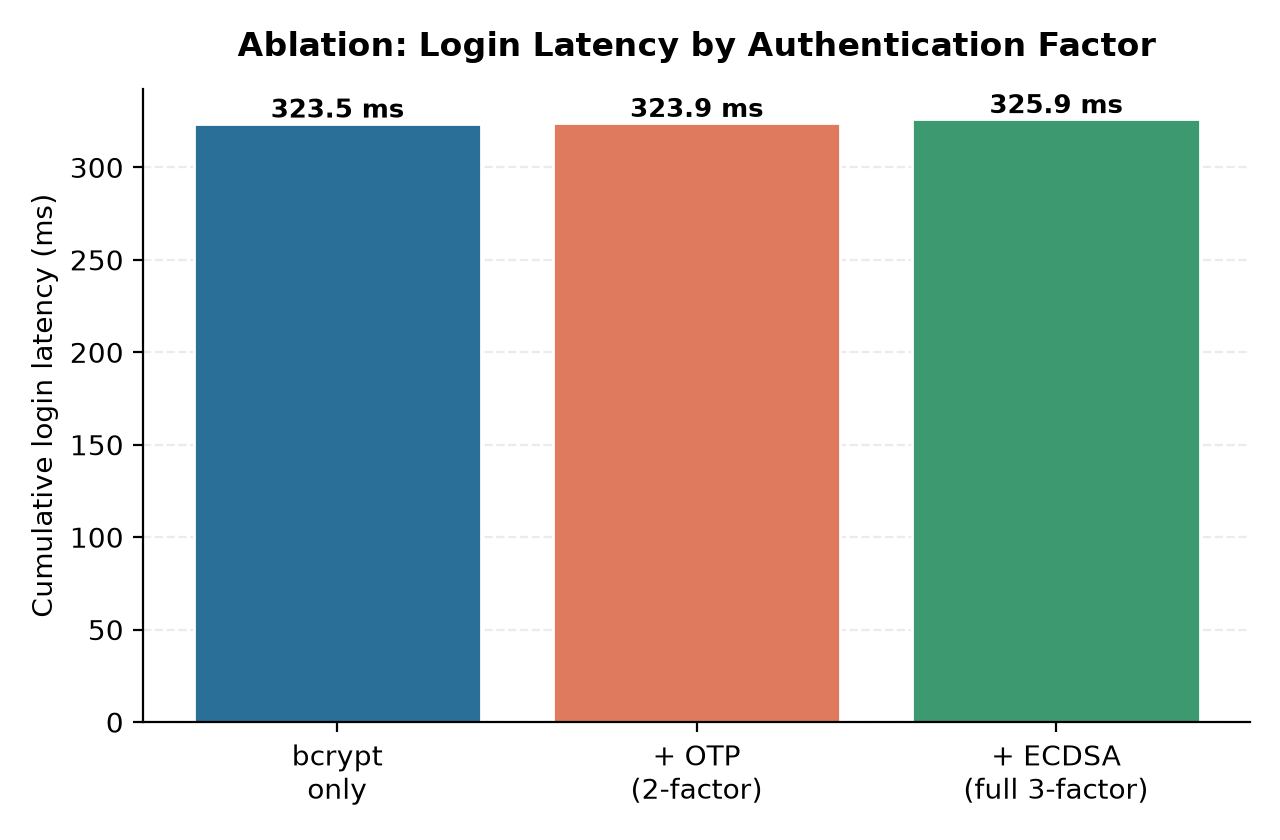
\includegraphics[width=0.47\textwidth]{figs/fig8_auth_ablation.png}
\caption{Cumulative administrator-login latency by authentication factor (all values measured).}
\label{fig:ablation}
\end{figure}

\subsection{Hyperparameter Tuning}
\label{sec:hyperparams}
Table~\ref{tab:hyperparams} records both the model and system constants for reproducibility.

\begin{table}[t]
\caption{Model and System Configuration Parameters}
\label{tab:hyperparams}
\centering
\small
\begin{tabular}{lc}
\toprule
\textbf{Parameter} & \textbf{Value} \\
\midrule
\multicolumn{2}{l}{\emph{Classifier}} \\
Backbone & ResNet-18 (ImageNet-pretrained) \\
Trainable layers & \texttt{layer4} + head \\
Input resolution $S$ & $224 \times 224$ \\
Batch size & 32 \\
Optimiser & AdamW \\
Learning rate $\eta$ & $3 \times 10^{-4}$ \\
Weight decay & $10^{-4}$ \\
LR schedule & Cosine annealing \\
Label smoothing $\varepsilon$ & 0.05 \\
Dropout & 0.3 \\
Class weighting & Inverse frequency (Eq.~\ref{eq:loss}) \\
Confidence threshold $\tau$ & 0.55 \\
Train/val/test split & 70 / 15 / 15 \\
\midrule
\multicolumn{2}{l}{\emph{Cryptography}} \\
bcrypt work factor $r$ & 12 ($2^{12}$ rounds) \\
AES key size & 256 bits \\
AES-GCM nonce size & 96 bits (12 bytes) \\
GCM authentication tag size & 128 bits (16 bytes) \\
CivicHash-512 output size & 512 bits (128 hex chars) \\
ECDSA curve & NIST P-256 (secp256r1) \\
OTP digit length $d_{\mathrm{len}}$ & 6 \\
JWT expiry (citizen / admin) & 2\,h / 8\,h \\
\midrule
\multicolumn{2}{l}{\emph{Geospatial}} \\
Boundary radius & 150\,km \\
Nominatim rate limit & 1 request/s \\
\bottomrule
\end{tabular}
\end{table}

\subsection{Security Architecture Strength}
The layered cryptographic architecture ensures no single point of compromise yields full system access: MongoDB alone yields only bcrypt hashes, encrypted images, and CivicHash-512 digests unreproducible without three independent secrets; the AES key file alone is insufficient to authenticate as an administrator without the ECDSA private key; a stolen password alone is insufficient without the private key from which the OTP is derived. This aligns with the multiple-independent-security-layer principle recommended by NIST \cite{grassi2017nist} and echoed in the benchmarking in \cite{l19ecdsabenchmark} recommendation of ECDSA P-256 for 128-bit-security deployments.

\subsection{The Cost of Removing the API}
Replacing hosted inference with an on-device classifier is a trade, and honesty requires stating both sides. What is gained: no API key or per-complaint cost; operation without connectivity; no citizen photograph leaving the server, which is consistent with the encrypt-at-rest guarantee the rest of the system makes; deterministic output, without which the integrity digest of Section~\ref{sec:module2} could not cover the complaint text at all; and a 69.9\,ms local inference in place of a network round-trip. What is lost: a general-purpose multimodal model can describe an arbitrary scene in open vocabulary, whereas our classifier is closed to seven categories and our descriptions are templated. A civic issue outside those seven categories will be forced into the nearest one --- mitigated, but not solved, by the confidence gate of Eq.~\ref{eq:confgate}.

\subsection{Real-World Usability}
CivicAI reduces the cognitive burden on citizen reporters by replacing manual form-filling with a photograph upload, closing the same feedback-loop gap identified in CPGRAMS \cite{rao2019cpgrams} and in \cite{l13citysolution, l14civicconnect}. Surfacing classifier confidence to the citizen, rather than hiding it, lets the person who actually observed the issue correct an uncertain categorisation before it reaches a department.

\subsection{Limitations}
Several limitations bound these results and should be read alongside them.

\emph{Dataset scale.} 1{,}373 images across seven categories is small. The training curves show clear overfitting, and the 82.76\% figure should be read as what transfer learning achieves under small-data conditions, not as a ceiling.

\emph{Training completeness.} The reported checkpoint is the best-validation model from a run that reached epoch 10 of a planned 15. Validation accuracy had plateaued (83.0\%$\rightarrow$85.9\% across those ten epochs) while training accuracy reached 99.9\%, so the remaining epochs would likely have yielded marginal change; nevertheless the schedule was not completed as specified.

\emph{Category separability.} \texttt{garbage} and \texttt{illegal\_dumping} overlap semantically to a degree that limits achievable accuracy regardless of model capacity. Merging them would raise category accuracy but discard a distinction with genuine municipal meaning --- illegal dumping is an enforcement matter, uncollected garbage a collection-schedule matter.

\emph{Templated descriptions.} Descriptions are drawn from category-conditioned templates and therefore describe the category rather than the specific photograph. A pothole 30\,cm deep and one 3\,cm deep receive the same text.

\emph{Key custody.} ECDSA private-key storage in the local \texttt{keys/} directory and the single AES master key file remain single points of failure appropriate for demonstration but not production, as also flagged for comparable centralised designs in \cite{l17decentralizedtrust}.

\emph{Session invalidation.} JWT tokens are not server-side invalidated upon logout, a risk class directly characterised by \cite{l20jwteemo}.

\emph{Single-machine evaluation.} All latencies are single-machine, single-user measurements. Concurrent-load behaviour is not characterised.

\section{Implementation}
\label{sec:implementation}

\subsection{Technology Stack}
The platform is implemented in Python 3.13. The web interface uses Gradio 6.26 with custom CSS. Data persistence employs MongoDB 8.0 via PyMongo 4.18 \cite{chodorow2013mongodb}. Classification uses PyTorch 2.6 with torchvision's ImageNet-pretrained ResNet-18; inference runs locally and requires no network access. Cryptographic operations use the Python \texttt{cryptography} library 50.x (OpenSSL backend) and \texttt{bcrypt} 5.0. Geospatial services query the OpenStreetMap Nominatim endpoint \cite{haklay2008osm} directly over HTTPS with client-side rate limiting and in-process caching. JWT tokens use a pure-Python HMAC-SHA256 implementation requiring no external JWT library \cite{jones2015jwt} --- a design choice reinforced by the analysis in \cite{l20jwteemo} finding that third-party JWT libraries are a common source of exploitable misconfiguration.

\subsection{Citizen Complaint Submission Flow}
The citizen flow proceeds as follows: (1) the citizen authenticates via bcrypt and receives a signed JWT; (2) the citizen uploads a photograph, optionally adds a note, and captures GPS location through the browser Geolocation API, with a manual address field as fallback when permission is denied; (3) coordinates are Haversine-validated (Eq.~\ref{eq:haversine}) and reverse-geocoded; (4) the image is normalised (Eq.~\ref{eq:resize}) and classified on-device (Eqs.~\ref{eq:softmax}--\ref{eq:argmax}), yielding category, department (Eq.~\ref{eq:routing}), title, description and confidence; (5) the raw image is encrypted with AES-256-GCM and the plaintext deleted; (6) the complaint is persisted with its CivicHash-512 digest over the location-inclusive field set (Eq.~\ref{eq:fieldset}); (7) the submission is written to the hash-chained audit log.

\subsection{Admin Authentication and Management Flow}
The administrator flow implements the three sequential security layers of Algorithm~\ref{alg:auth}, specified in Section~\ref{sec:module3}. Only upon passing all three does the server issue an admin-scoped JWT. Administrators view all complaints with per-record CivicHash-512 integrity status, reported location with a map link, and classifier confidence; update complaint statuses; and view complaint images decrypted in memory only. Every status transition recomputes the record's digest under its own hash version, writes an audit entry, and creates a citizen notification. The citizen dashboard polls for these changes, so a status update propagates without requiring re-authentication.

\subsection{Security Audit Logging}
The dual-output logger writes every security-relevant event --- \texttt{LOGIN\_SUCCESS}, \texttt{LOGIN\_FAILED}, \texttt{IMAGE\_ENCRYPTED}, \texttt{IMAGE\_DECRYPTED}, \texttt{COMPLAINT\_SUBMITTED}, \texttt{COMPLAINT\_CLASSIFIED}, \texttt{STATUS\_UPDATED}, \texttt{ADMIN\_CREDENTIALS\_RESET} --- to the filesystem and to MongoDB, hash-chained per Eq.~\ref{eq:auditchain}. Chain state is guarded by a mutex so concurrent requests cannot compute their hashes from the same predecessor.

\section{Conclusion and Future Work}
\label{sec:conclusion}
This paper presented CivicAI, a cryptographically secured civic issue reporting platform whose visual categorisation runs entirely on-device. Replacing the hosted multimodal-LLM stage with a transfer-learned ResNet-18 removed the external API dependency, the per-complaint cost and the connectivity requirement --- and, more fundamentally, made the generated complaint text deterministic, which is a precondition for binding that text into a cryptographic integrity digest at all.

% <<<AUTO:conclusion_results>>>
Measured on 203 held-out images, the 2-member ensemble (resnet50 and efficientnet-b0) attains 84.73\% category accuracy, 0.839 macro-F1 and 0.976 mean AUC. Because the category-to-department routing table maps visually confusable categories onto shared departments, department-routing accuracy reaches 90.15\% --- and we argue this is the metric civic-classification work should report, since it is what determines whether a complaint is actioned.
% <<<END:conclusion_results>>>

In the cryptographic domain, CivicHash-512 combines AES-256-GCM, HMAC-SHA256 and triple-round SHA-512 into a three-secret-bound 512-bit digest computed in 0.213\,ms, now covering the reported GPS location so a complaint cannot be silently relocated in the database. The audit log's hash chain was verified to detect and localise a single-character modification. Complete cryptographic protection of one complaint costs 17.1\,ms against 69.9\,ms for classification: in this system, securing a report is four times cheaper than understanding it.

\subsection{Future Work}
\begin{itemize}
\item Expansion of the training corpus, with particular attention to the \texttt{garbage}/\texttt{illegal\_dumping} boundary, and completion of the full training schedule.
\item Severity estimation in addition to categorisation, so descriptions reflect the specific photograph rather than the category, following the size-estimation approach of \cite{l2enhancedyolo}.
\item Detection of AI-generated or otherwise fabricated evidence photographs, an attack surface no surveyed system addresses and one that grows as image synthesis becomes commonplace.
\item An independent cryptographic audit of CivicHash-512, following the benchmarking rigour demonstrated in \cite{l19ecdsabenchmark}.
\item Migration of AES and ECDSA key storage to a dedicated secrets-management service, and server-side JWT revocation.
\item A mobile-native companion application with background GPS tracking.
\item Adoption of a lightweight, domain-specific ledger such as SC-Chain \cite{l16scchain} for the audit-log layer, should decentralisation become a requirement.
\item Concurrent-load scalability characterisation.
\end{itemize}

\section*{Acknowledgment}
The authors thank the Department of Computer Science and Engineering, VIT University, Chennai, for providing the infrastructure and academic guidance that supported this work. This project was developed as part of the course CNS BCSE309P --- Cryptography and Network Security.

\begin{thebibliography}{99}

\bibitem{zhang2021resnet} Y. Zhang, L. Wang, and Q. Liu, ``Deep learning-based pothole detection on urban roads using ResNet-50,'' \emph{IEEE Trans. Intell. Transp. Syst.}, vol. 22, no. 8, pp. 4914--4925, Aug. 2021.
\bibitem{majumdar2020yolov4} S. Majumdar, A. Roy, and P. Ghosh, ``Real-time garbage detection in urban environments using YOLOv4,'' in \emph{Proc. IEEE Int. Conf. Smart Structures and Systems (ICSSS)}, 2020, pp. 1--6.
\bibitem{almahmoud2023bert} M. Almahmoud, R. Alotaibi, and H. Alshehri, ``BERT-based automated civic complaint routing for smart city platforms,'' \emph{IEEE Access}, vol. 11, pp. 32541--32553, 2023.
\bibitem{offenhuber2017waste} D. Offenhuber, \emph{Waste Is Information: Infrastructure Legibility and Governance}. Cambridge, MA: MIT Press, 2017.
\bibitem{rao2019cpgrams} K. Rao, N. Sharma, and A. Joshi, ``Evaluation of CPGRAMS: India's centralized public grievance redress system,'' \emph{J. e-Governance}, vol. 42, no. 1, pp. 51--64, 2019.
\bibitem{bonneau2012passwords} J. Bonneau, C. Herley, P. C. van Oorschot, and F. Stajano, ``The quest to replace passwords: A framework for comparative evaluation of web authentication schemes,'' in \emph{Proc. IEEE Symp. Security and Privacy}, 2012, pp. 553--567.
\bibitem{krawczyk1997hmac} H. Krawczyk, ``HMAC: Keyed-hashing for message authentication,'' IETF RFC 2104, Feb. 1997.
\bibitem{mcgrew2004gcm} D. A. McGrew and J. Viega, ``The Galois/Counter Mode of operation (GCM),'' NIST Submission, 2004.
\bibitem{provos1999bcrypt} N. Provos and D. Mazi\`eres, ``A future-adaptable password scheme,'' in \emph{Proc. USENIX Annual Technical Conf.}, 1999, pp. 81--91.
\bibitem{nist2023fips186} National Institute of Standards and Technology, ``Digital Signature Standard (DSS), FIPS PUB 186-5,'' NIST, Gaithersburg, MD, Feb. 2023.
\bibitem{touvron2023llama} H. Touvron et al., ``LLaMA: Open and efficient foundation language models,'' arXiv preprint arXiv:2302.13971, 2023.
\bibitem{haklay2008osm} M. Haklay and P. Weber, ``OpenStreetMap: User-generated street maps,'' \emph{IEEE Pervasive Comput.}, vol. 7, no. 4, pp. 12--18, Oct. 2008.
\bibitem{bellare1996keying} M. Bellare, R. Canetti, and H. Krawczyk, ``Keying hash functions for message authentication,'' in \emph{Advances in Cryptology --- CRYPTO 1996}, LNCS vol. 1109, Springer, 1996, pp. 1--15.
\bibitem{ahmed2021pothole} K. R. Ahmed, ``Smart pothole detection using deep learning based on dilated convolution,'' \emph{Sensors}, vol. 21, no. 24, art. no. 8406, Dec. 2021.
\bibitem{goyal2023blockchain} S. Goyal, P. Bedi, J. Kumar, and V. Sharma, ``Smart city complaint management system using blockchain and AI for transparent civic governance,'' \emph{Smart Cities}, vol. 6, no. 2, pp. 1045--1063, 2023.
\bibitem{stallings2017crypto} W. Stallings, \emph{Cryptography and Network Security: Principles and Practice}, 7th ed. Hoboken, NJ: Pearson, 2017.
\bibitem{johnson2001ecdsa} D. Johnson, A. Menezes, and S. Vanstone, ``The Elliptic Curve Digital Signature Algorithm (ECDSA),'' \emph{Int. J. Inf. Secur.}, vol. 1, no. 1, pp. 36--63, 2001.
\bibitem{islam2022cloud} M. S. Islam, M. R. Islam, and M. S. H. Khan, ``A comprehensive review of secure cloud storage using AES encryption and cryptographic integrity mechanisms,'' \emph{J. Inf. Secur. Appl.}, vol. 65, art. no. 103117, 2022.
\bibitem{jones2015jwt} M. Jones, J. Bradley, and N. Sakimura, ``JSON Web Token (JWT),'' IETF RFC 7519, May 2015.
\bibitem{grassi2017nist} P. A. Grassi et al., ``Digital identity guidelines: Authentication and lifecycle management, NIST Special Publication 800-63B,'' NIST, Gaithersburg, MD, Jun. 2017.
\bibitem{chodorow2013mongodb} K. Chodorow, \emph{MongoDB: The Definitive Guide}, 2nd ed. Sebastopol, CA: O'Reilly Media, 2013.
\bibitem{he2016resnet} K. He, X. Zhang, S. Ren, and J. Sun, ``Deep residual learning for image recognition,'' in \emph{Proc. IEEE Conf. Computer Vision and Pattern Recognition (CVPR)}, 2016, pp. 770--778.
\bibitem{deng2009imagenet} J. Deng, W. Dong, R. Socher, L.-J. Li, K. Li, and L. Fei-Fei, ``ImageNet: A large-scale hierarchical image database,'' in \emph{Proc. IEEE CVPR}, 2009, pp. 248--255.
\bibitem{loshchilov2019adamw} I. Loshchilov and F. Hutter, ``Decoupled weight decay regularization,'' in \emph{Proc. Int. Conf. Learning Representations (ICLR)}, 2019.
\bibitem{szegedy2016labelsmooth} C. Szegedy, V. Vanhoucke, S. Ioffe, J. Shlens, and Z. Wojna, ``Rethinking the Inception architecture for computer vision,'' in \emph{Proc. IEEE CVPR}, 2016, pp. 2818--2826.
\bibitem{l1potyolo} Bhavana et al., ``POT-YOLO: Real-Time Road Potholes Detection Using Edge Segmentation-Based YOLOv8 Network,'' \emph{IEEE Sensors J.}, 2024.
\bibitem{l2enhancedyolo} ``An Enhanced YOLOv8 Model for Real-Time and Accurate Pothole Detection and Size Estimation,'' 2025.
\bibitem{l3roadperception} ``Road Perception for Autonomous Driving: Pothole Detection in Complex Environments Based on Improved YOLOv8,'' \emph{IEEE J. Mag.}, 2024--2025.
\bibitem{l4realtimepothole} ``Real-time Potholes Detection and Localization using YOLOv8,'' \emph{IEEE Conf. Publ.}, 2024.
\bibitem{l5multiclasswaste} ``Deep Learning Based Multi-Class Waste Object Detection and Classification,'' \emph{IEEE Conf. Publ.}, 2024--2025.
\bibitem{l6householdgarbage} ``Application research of image classification algorithm based on deep learning in household garbage sorting,'' 2024.
\bibitem{l7belugawaste} ``Intelligent and sustainable waste classification model based on multi-objective beluga whale optimization and deep learning,'' \emph{Environ. Sci. Pollut. Res.}, 2024.
\bibitem{l8visualpollution} ``A Scoping Review of Deep Learning for Urban Visual Pollution and Proposal of a Real-Time Monitoring Framework with a Visual Pollution Index,'' 2025--2026.
\bibitem{l9mllmaudit} ``Multimodal Large Language Models as Built Environment Auditing Tools,'' \emph{Professional Geographer}, 2024.
\bibitem{l10quantizedvlm} ``Quantized Vision-Language Models for Damage Assessment: A Comparative Study of LLaVA-1.5-7B Quantization Levels,'' 2025--2026.
\bibitem{l11llmearthquake} ``Large Language Model for Post-Earthquake Structural Damage Assessment of Buildings,'' \emph{Comput.-Aided Civ. Infrastruct. Eng.}, 2025.
\bibitem{l12urbanllava} ``UrbanLLaVA: A Multi-modal Large Language Model for Urban Intelligence with Spatial Reasoning and Understanding,'' 2025.
\bibitem{l13citysolution} F. Shama, A. Aziz, and L. B. M. Deya, ``CitySolution: A complaining task distributive mobile application for smart city corporation using deep learning,'' 2024.
\bibitem{l14civicconnect} J. Sowjanya, D. Deekshith, T. Ritwik, and V. S. V. V. Daketi, ``CivicConnect: A Geo-Spatially Enabled Smart Civic Issue Reporting and Proof-Based Resolution System,'' \emph{Int. J. Eng. Techniques}, vol. 12, no. 3, 2026.
\bibitem{l15grievanceblockchain} ``An Analytical Study on the Efficacy of Blockchain Frameworks for Student Grievance Management,'' \emph{SN Comput. Sci.}, 2024.
\bibitem{l16scchain} K. Fan et al., ``SC-Chain: An efficient blockchain framework for smart city,'' \emph{IEEE Internet Things J.}, vol. 11, pp. 7863--7877, 2024.
\bibitem{l17decentralizedtrust} ``Decentralized trust framework for smart cities: a blockchain-enabled cybersecurity and data integrity model,'' \emph{Sci. Rep.}, 2025.
\bibitem{l18pqcsession} ``Design and implementation of an authenticated post-quantum session protocol using ML-KEM (Kyber), ML-DSA (Dilithium), and AES-256-GCM,'' \emph{Frontiers in Physics}, 2025.
\bibitem{l19ecdsabenchmark} ``Towards Sustainable and Trustworthy Digital Infrastructure: Benchmarking RSA and ECDSA Digital Signature Algorithms in Support of SDGs 9 and 16,'' 2025.
\bibitem{l20jwteemo} ``Token Time Bomb: Evaluating JWT Implementations for Vulnerability Discovery,'' \emph{Proc. NDSS}, 2026.

\end{thebibliography}

\end{document}
